% Created 2024-01-09 Tue 09:17
% Intended LaTeX compiler: pdflatex
\documentclass[a4paper,11pt,twoside]{article}
\usepackage[utf8]{inputenc}
\usepackage[T1]{fontenc}
\usepackage{graphicx}
\usepackage{longtable}
\usepackage{wrapfig}
\usepackage{rotating}
\usepackage[normalem]{ulem}
\usepackage{amsmath}
\usepackage{amssymb}
\usepackage{capt-of}
\usepackage{hyperref}
\usepackage{listings}
\usepackage{helvet}
\usepackage{longtable}
\usepackage[margin=0.5in]{geometry}
\renewcommand\familydefault{\sfdefault}
\setlength{\textheight}{230mm}
\setlength{\textwidth}{160mm}
\setlength{\oddsidemargin}{0mm}
\setlength{\evensidemargin}{0mm}
\addtolength{\parskip}{0.33\baselineskip}
\setlength\parindent{0pt}
\usepackage[inline]{enumitem}
\setlist{nosep}
\usepackage[x11names]{xcolor}
\usepackage{tabularx}
\hypersetup{linktoc = all, colorlinks = true, urlcolor = DodgerBlue4, citecolor = PaleGreen1, linkcolor = black}
\date{\today}
\title{Hiqa Inspection Reports - Data Aggregation \& Analysis\\\medskip
\large Draft First Look}
\hypersetup{
 pdfauthor={Eoin Carney},
 pdftitle={Hiqa Inspection Reports - Data Aggregation \& Analysis},
 pdfkeywords={},
 pdfsubject={},
 pdfcreator={Emacs 29.1 (Org mode 9.7)}, 
 pdflang={English}}
\begin{document}

\maketitle
\tableofcontents

\clearpage
\section{Context and Method}
\label{sec:org4230c98}
The data below was taken from the \href{https://www.hiqa.ie/reports-and-publications/inspection-reports}{HIQA Inspection Reports} for Disability Centres, available on their website in \texttt{.pdf} format.

Report URLs are listed under pages for \href{https://www.hiqa.ie/find-a-centre}{centres} where an inspection has occurred (\href{https://www.hiqa.ie/areas-we-work/find-a-centre/st-dominics-services}{example}). Using the HIQA register for disability centres, it was possible to get the URLs for the centre pages, and from these, the URLs for related inspection  reports.

Reports are written according to a standard template, making them relatively easy to parse. For the extraction, four main areas of the report were focused on:

\begin{itemize}
\item \textbf{``Frontmatter''} area on the first page, including details of the centre id, date of inspection, type of inspection, etc.
\item \textbf{Number of residents present} at the time of inspection
\item Levels of \textbf{compliance} for the regulations inspected (``Compliant'', ``Not compliant'', ``Substantially compliant'')
\item The narrative text from the section titled ``\textbf{What residents told us and what inspectors observed}''
\end{itemize}

This is not an exhaustive list of information that could be extracted from the reports.

As part of this process 3,179 Inspection Reports were gathered/parsed. This compares with 3,312 that appear to be available on the HIQA website (as at 30\textsuperscript{th} December, 2023). In other words, the data covers about 96\% of the Inspection Reports for Disability Centres. In the case of the field ``Number of Residents Present'', there were 41 missing entries out of the 3,179 reports. Upon further inspection, the reason for this appears to be the introduction of a new type of report in 2023; ``Report of a Restrictive Practice Thematic Inspection''. See example \href{https://www.hiqa.ie/system/files?file=inspectionreports/5654-an-diadan-26-september-2023.pdf}{here}. These reports do not record number of residents present, nor compliance with the various regulations. Instead, there is an overall judgment based on the specific criteria of these reports. These specific judgements for thematic inspection reports were not captured here.

The dates of the reports range from \textbf{3\textsuperscript{rd} June 2020} - \textbf{18\textsuperscript{th} October 2023}.
\section{Number of Inspections}
\label{sec:orgeba7e1a}
Between 2020 and 2023, there were:

\begin{itemize}
\item \textbf{3,179} inspection reports
\item \textbf{1,333} centres
\item \textbf{94} providers
\item \textbf{38,330} total checks for compliance
\end{itemize}

For the years 2021 and 2022, the average number of inspections per month was \textbf{86}.

\begin{center}
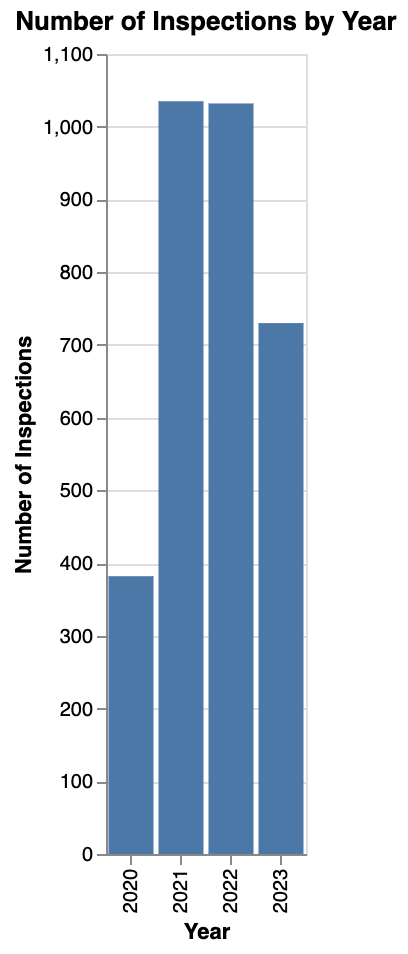
\includegraphics[height=0.7\textwidth]{img/01_inspections_by_year.png}
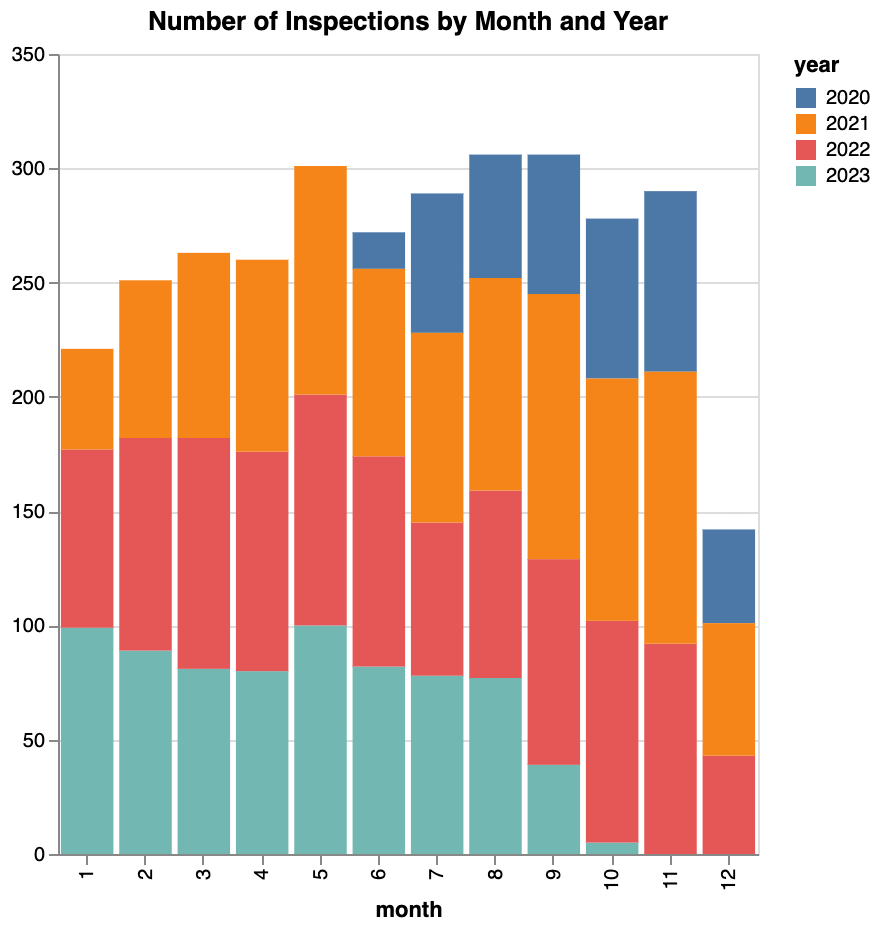
\includegraphics[height=0.7\textwidth]{img/02_inspections_by_month.png}
\end{center}
\section{Number of Inspections per Centre}
\label{sec:org953ae41}
A significant majority (\textbf{78\%}) of centres received either 2 or 3 inspections over the period covered by the reports.

\begin{longtable}{rr}
\caption{Number of Inspections per Centre 2020-2023}
\\[0pt]
Number of Inspections & Number of Centres\\[0pt]
\hline
\endfirsthead
\multicolumn{2}{l}{Continued from previous page} \\[0pt]
\hline

Number of Inspections & Number of Centres \\[0pt]

\hline
\endhead
\hline\multicolumn{2}{r}{Continued on next page} \\
\endfoot
\endlastfoot
\hline
1 & 168\\[0pt]
2 & 636\\[0pt]
3 & 415\\[0pt]
4 & 84\\[0pt]
5 & 23\\[0pt]
6 & 6\\[0pt]
7 & 1\\[0pt]
\end{longtable}

\clearpage
\begin{longtable}{rrrr}
\caption{Number of Inspections per Centre by Year}
\\[0pt]
Year & 1 Inspection & 2 Inspections & 3 Inspections\\[0pt]
\hline
\endfirsthead
\multicolumn{4}{l}{Continued from previous page} \\[0pt]
\hline

Year & 1 Inspection & 2 Inspections & 3 Inspections \\[0pt]

\hline
\endhead
\hline\multicolumn{4}{r}{Continued on next page} \\
\endfoot
\endlastfoot
\hline
2020 & 367 & 6 & 1\\[0pt]
2021 & 883 & 73 & 2\\[0pt]
2022 & 817 & 94 & 9\\[0pt]
2023 & 655 & 36 & 1\\[0pt]
\end{longtable}
\section{Number of Residents Present}
\label{sec:org6f0886d}

The number of residents present at the time of inspection is highly contingent, so any clear line drawn between 'number of residents present' and actual 'occupancy' level of the centres is difficult. For example, there were 19 centres with '0' residents present at time of inspection. The HIQA register also lists \textbf{maximum occupancy} for a centre. Therefore, the true 'number of residents' would be somewhere between residents present for the inspection and maximum occupancy. To complicate things further, there were a number of centres which had \emph{more} residents present compared to the 'maximum occupancy' as listed in the HIQA register, for example, \href{https://www.hiqa.ie/areas-we-work/find-a-centre/grove-1}{see this centre and corresponding inspection report}.

Figures relating to 'number of residents present' were taken from the \emph{most recent} inspection report where there were multiple inspections per centre.
\begin{itemize}
\item The total number of residents present across the reports was \textbf{7,517}
\item The total maximum occupancy according to the HIQA register is \textbf{9,126}
\end{itemize}
\subsection{Distribution - Residents Present and Maximum Occupancy}
\label{sec:org7dee06e}
The majority of centres had \textbf{4} residents present at time of inspection.

\begin{center}
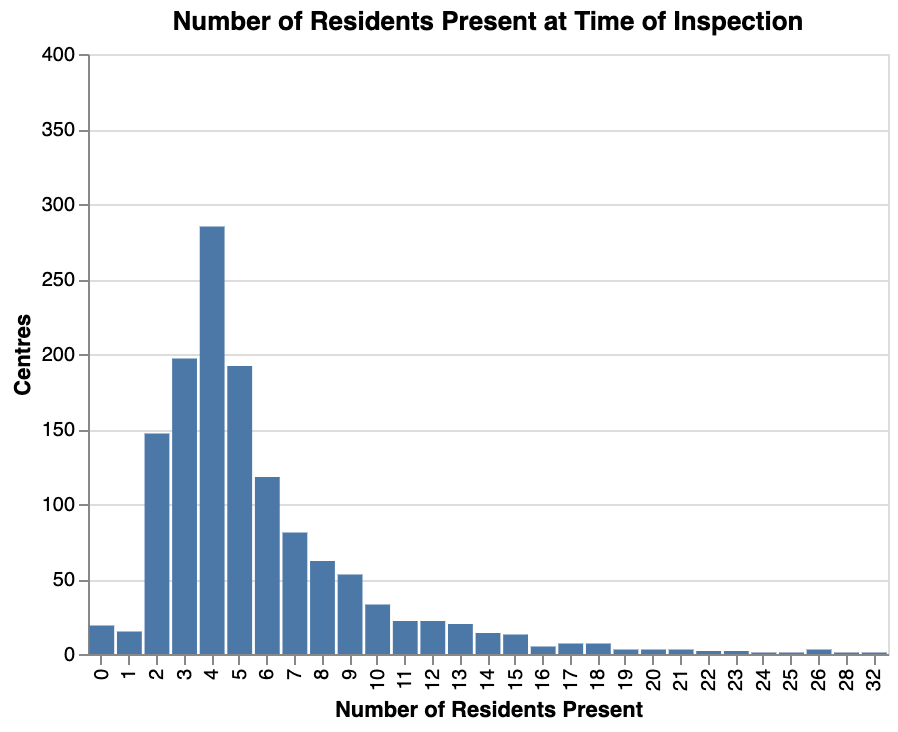
\includegraphics[width=10cm]{img/03_no_residents_dist.png}
\end{center}
\begin{center}
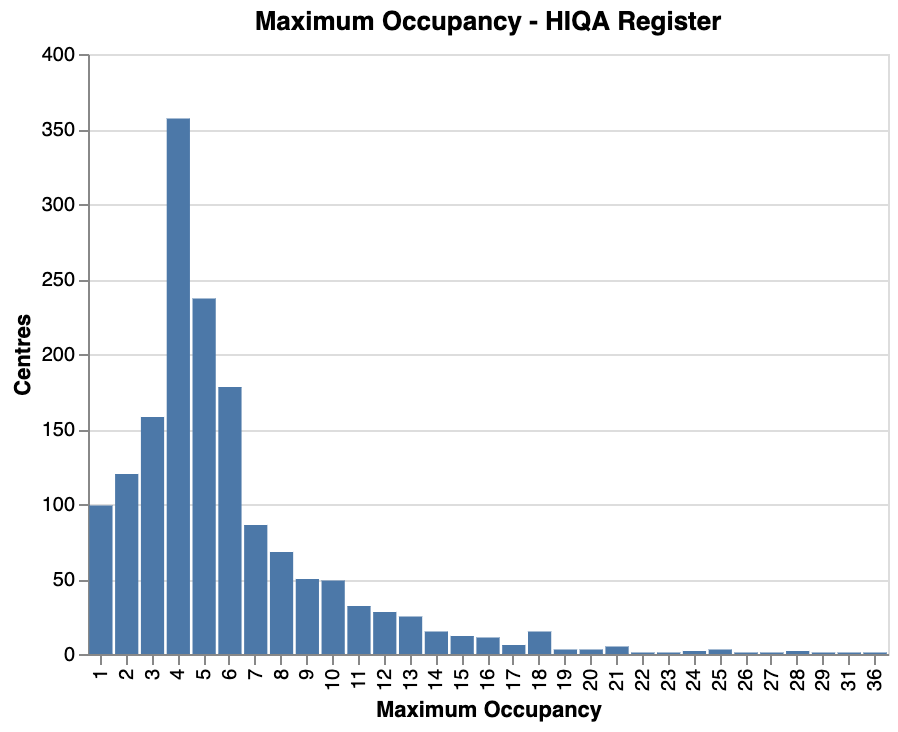
\includegraphics[width=10cm]{img/04_max_occupancy_dist.png}
\end{center}
\subsection{Average Residents Present by Area}
\label{sec:org9965c4f}

On average, \textbf{Cork} had the most residents present per centre.

\begin{center}
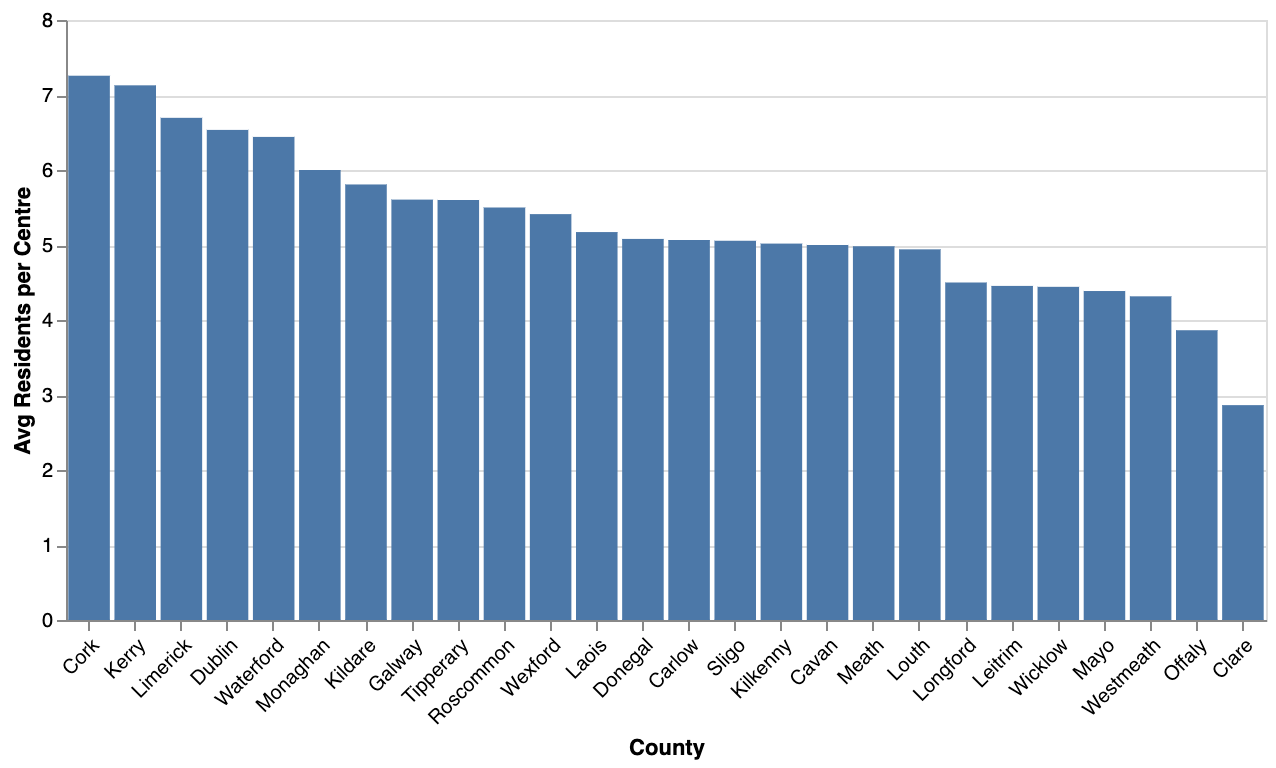
\includegraphics[width=.9\linewidth]{img/06_01_avg_res_per_centre.png}
\end{center}
\subsection{Congregated and Decongregated Settings}
\label{sec:orga62c0b8}

As part of the \href{https://www.hse.ie/eng/services/list/4/disability/congregatedsettings/timetomoveon.html\#:\~:text=Time\%20to\%20Move\%20on\%20from\%20Congregated\%20Settings\%20\%E2\%80\%93,people\%20to\%20\%E2\%80\%98live\%20ordinary\%20lives\%20in\%20ordinary\%20places\%E2\%80\%99.}{Time to Move on From Congregated Settings} policy, there is a commitment to moving people out from congregated settings where there are 10 or more people living together to ordinary homes where no more than 4 individuals live together. Using the ``number of residents'' present at an inspection and the HIQA registers' ``Maximum Occupancy'' information, it is possible to get a sense of the split between centres with \textbf{10+} people and centres with \textbf{less than 10 people}.

Based on ``number of residents present'', \textbf{70\%} of people lived centres with less than 10 people. Based on the HIQA register, \textbf{66\%} of the maximum occupancy is related to centres with less than 10.

This corresponds to \textbf{163} (\textbf{14\%}) congregated centres aligned to 'number of residents present', and \textbf{218} congregated centres (in terms of capacity) according to the HIQA registers' 'maximum occupancy'

\begin{center}
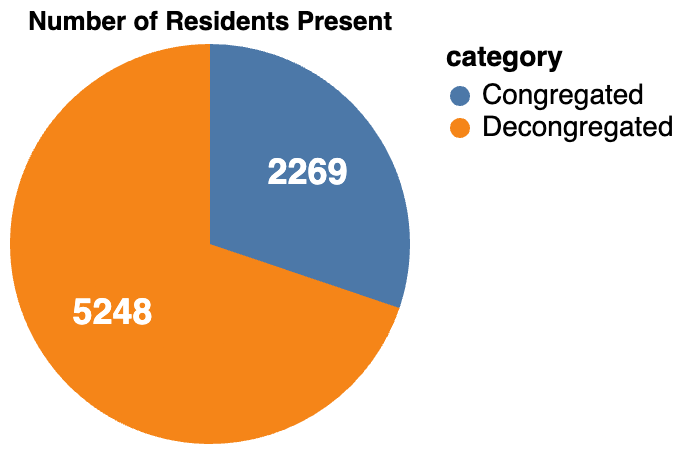
\includegraphics[height=0.3\textwidth]{img/05_num_residents_congregated.png}
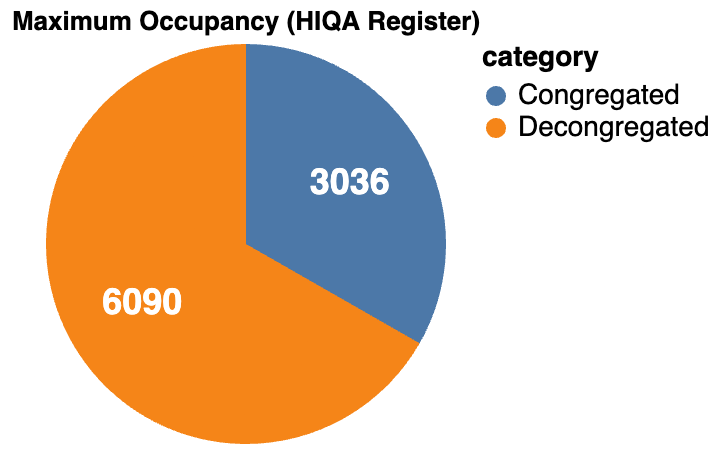
\includegraphics[height=0.3\textwidth]{img/06_max_occ_congregated.png}
\end{center}

\begin{longtable}{lrr}
\caption{Residents Present - levels of decongregation}
\\[0pt]
Category & Number of Residents Present & Number of Centres\\[0pt]
\hline
\endfirsthead
\multicolumn{3}{l}{Continued from previous page} \\[0pt]
\hline

Category & Number of Residents Present & Number of Centres \\[0pt]

\hline
\endhead
\hline\multicolumn{3}{r}{Continued on next page} \\
\endfoot
\endlastfoot
\hline
4 or less & 2040 & 663\\[0pt]
Between 5 and 9 & 3208 & 506\\[0pt]
10 or more & 2269 & 163\\[0pt]
\end{longtable}


\clearpage
\section{Compliance Levels}
\label{sec:orgd8c7dc8}
There are 32 regulations that can be checked as part of inspections. Not every inspection checks for compliance against all regulations. On average, \textbf{12} regulations were checked per inspection. Compliance is listed as either ``Compliant'', ``Substantially compliant'' or ``Not compliant''.

The following regulations relate to the area of \textbf{Capacity and Capability}:

\begin{itemize}
\item Regulation 3: Statement of purpose
\item Regulation 4: Written policies and procedures
\item Regulation 14: Person in charge
\item Regulation 15: Staffing
\item Regulation 16: Training and staff development
\item Regulation 19: Directory of residents
\item Regulation 21: Records
\item Regulation 22: Insurance
\item Regulation 23: Governance and management
\item Regulation 24: Admissions and contract for the provision of services
\item Regulation 30: Volunteers
\item Regulation 31: Notification of incidents
\item Regulation 32: Notifications of periods when person in charge is absent
\item Regulation 33: Notifications of procedures and arrangements for periods when person in charge is absent
\item Regulation 34: Complaints procedure
\end{itemize}

The following regulations relate to \textbf{Quality and Safety}:

\begin{itemize}
\item Regulation 5: Individualised assessment and personal plan
\item Regulation 6: Healthcare
\item Regulation 7: Positive behaviour support
\item Regulation 8: Protection
\item Regulation 9: Residents' rights
\item Regulation 10: Communication
\item Regulation 11: Visits
\item Regulation 12: Personal possessions
\item Regulation 13: General welfare and development
\item Regulation 17: Premises
\item Regulation 18: Food and nutrition
\item Regulation 20: Information for residents
\item Regulation 25: Temporary absence, transition and discharge of residents
\item Regulation 26: Risk management procedures
\item Regulation 27: Protections against infection
\item Regulation 28: Fire precautions
\item Regulation 29: Medicines and pharmaceutical services
\end{itemize}

The rate of non-compliant regulations stayed mostly stable at around 10-11\% per year.

\begin{longtable}{rrrr}
\caption{Regulation Compliance by Year}
\\[0pt]
Year & Compliant & Substantially compliant & Not compliant\\[0pt]
\hline
\endfirsthead
\multicolumn{4}{l}{Continued from previous page} \\[0pt]
\hline

Year & Compliant & Substantially compliant & Not compliant \\[0pt]

\hline
\endhead
\hline\multicolumn{4}{r}{Continued on next page} \\
\endfoot
\endlastfoot
\hline
2023 & 6020 & 1615 & 941\\[0pt]
2022 & 6340 & 2546 & 1078\\[0pt]
2021 & 10303 & 2799 & 1448\\[0pt]
2020 & 3747 & 930 & 563\\[0pt]
\end{longtable}

\begin{center}
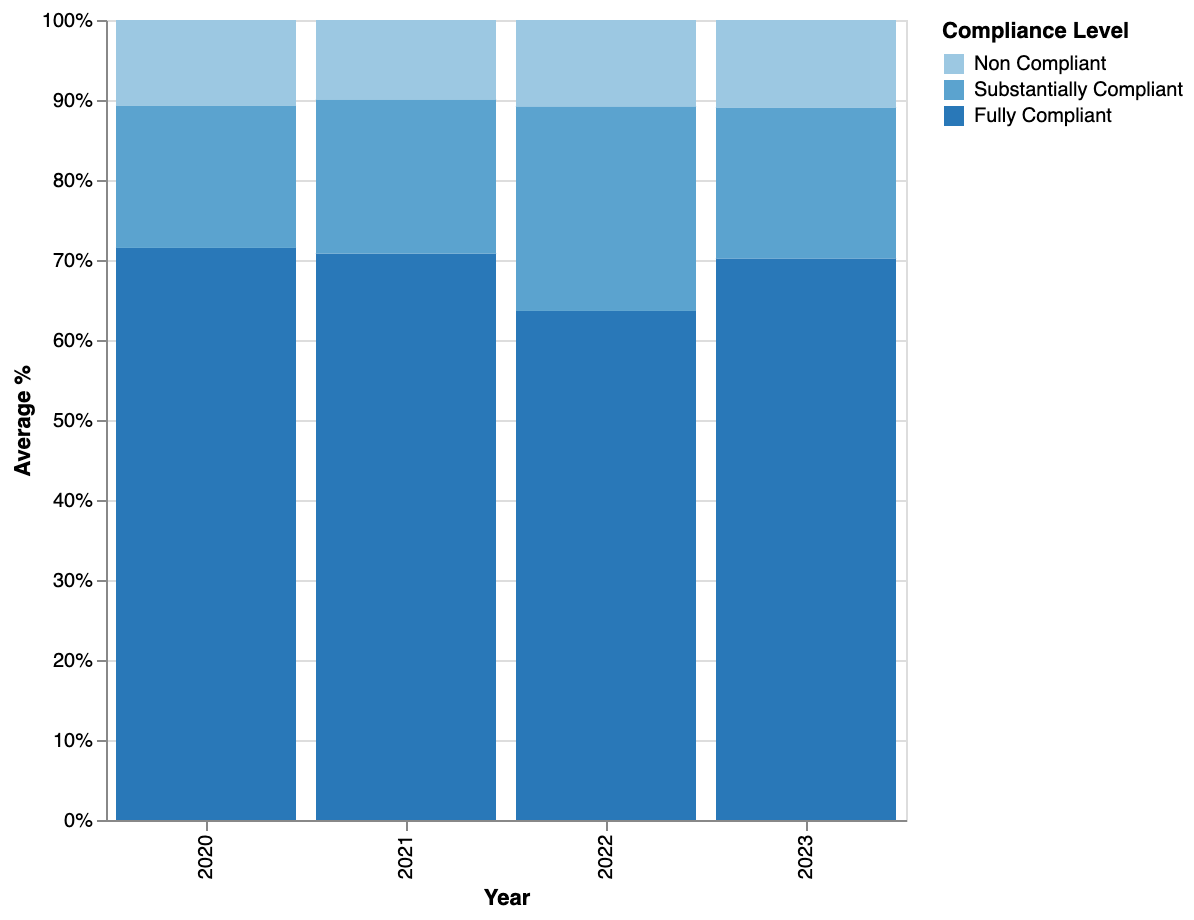
\includegraphics[width=.9\linewidth]{img/07_compliance_by_year.png}
\end{center}

The most checked capacity and capability regulation across the reports was regulation 23, \textbf{governance and management}, which also had the highest rate of non compliance.

The most checked quality and safety regulation across the reports was regulation 27, \textbf{protections against infection}. The regulation with the highest rate of non-compliance for quality and safety was regulation 28, \textbf{Fire precautions}.

\clearpage
\begin{longtable}{lrr}
\caption{Capacity and Capability Regulations NonCompliance Rate 2020-2023}
\\[0pt]
Regulation & Total Inspections & \% Not Compliant\\[0pt]
\hline
\endfirsthead
\multicolumn{3}{l}{Continued from previous page} \\[0pt]
\hline

Regulation & Total Inspections & \% Not Compliant \\[0pt]

\hline
\endhead
\hline\multicolumn{3}{r}{Continued on next page} \\
\endfoot
\endlastfoot
\hline
Governance and management & 2648 & 20.62\\[0pt]
Staffing & 2530 & 12.65\\[0pt]
Training and staff development & 2267 & 9.00\\[0pt]
Person in charge & 1616 & 2.85\\[0pt]
Notification of incidents & 1498 & 19.63\\[0pt]
Statement of purpose & 1424 & 2.32\\[0pt]
Complaints procedure & 1082 & 5.91\\[0pt]
Admissions and contract for the provision of services & 597 & 14.57\\[0pt]
Directory of residents & 409 & 1.71\\[0pt]
Written policies and procedures & 333 & 11.71\\[0pt]
Records & 266 & 13.53\\[0pt]
Notifications of periods when person in charge is absent & 50 & 16.00\\[0pt]
\end{longtable}


\begin{longtable}{lrr}
\caption{Quality and Safety Regulations NonCompliance Rate 2020-2023}
\\[0pt]
Regulation & Total Inspections & \% Not Compliant\\[0pt]
\hline
\endfirsthead
\multicolumn{3}{l}{Continued from previous page} \\[0pt]
\hline

Regulation & Total Inspections & \% Not Compliant \\[0pt]

\hline
\endhead
\hline\multicolumn{3}{r}{Continued on next page} \\
\endfoot
\endlastfoot
\hline
Protections against infection & 2775 & 11.78\\[0pt]
Protection & 2295 & 8.89\\[0pt]
Individualised assessment and personal plan & 2236 & 9.66\\[0pt]
Risk management procedures & 2123 & 8.43\\[0pt]
Fire precautions & 2121 & 19.14\\[0pt]
Premises & 2077 & 16.51\\[0pt]
Positive behaviour support & 1800 & 9.22\\[0pt]
Healthcare & 1754 & 2.74\\[0pt]
Residents' rights & 1661 & 12.04\\[0pt]
General welfare and development & 1007 & 6.95\\[0pt]
Medicines and pharmaceutical services & 609 & 12.15\\[0pt]
Communication & 565 & 1.42\\[0pt]
Information for residents & 547 & 0.37\\[0pt]
Food and nutrition & 449 & 2.67\\[0pt]
Personal possessions & 411 & 16.79\\[0pt]
Visits & 388 & 1.55\\[0pt]
Temporary absence, transition and discharge of residents & 184 & 8.70\\[0pt]
\end{longtable}

\clearpage

\begin{center}
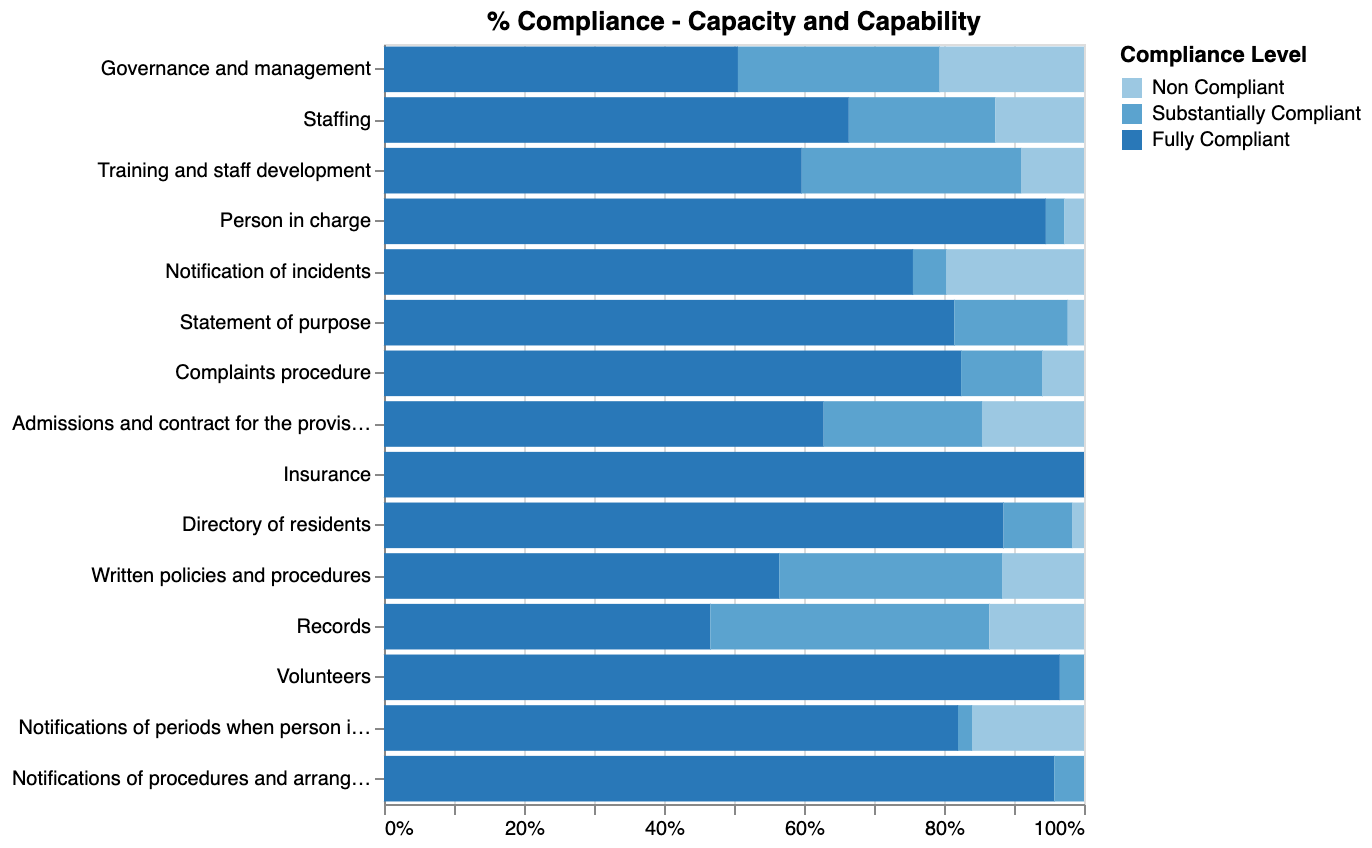
\includegraphics[width=.9\linewidth]{img/08_compliance_capacity.png}
\end{center}

\begin{center}
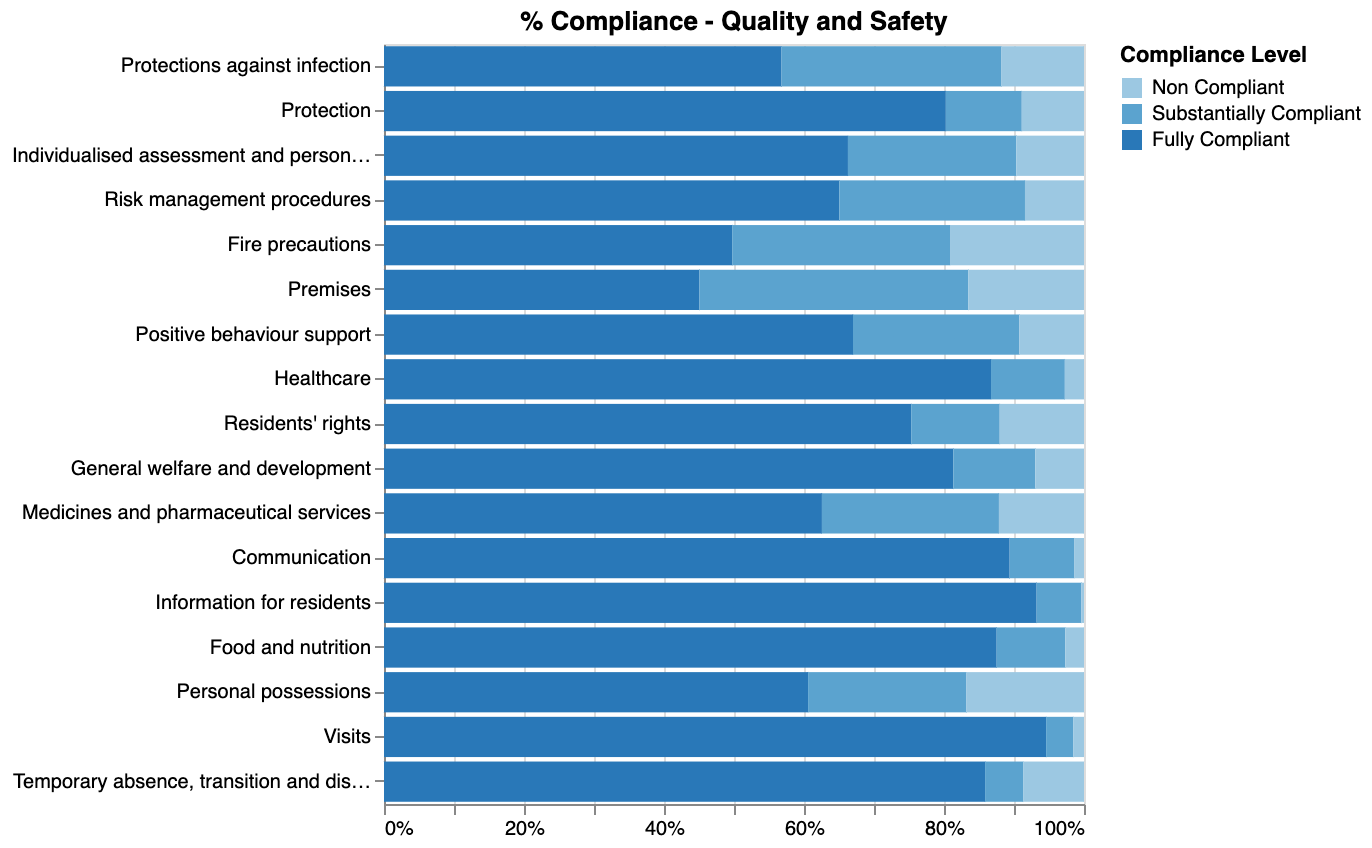
\includegraphics[width=.9\linewidth]{img/09_compliance_quality.png}
\end{center}
\subsection{Compliance by Provider}
\label{sec:org739211e}
As mentioned above, there were 94 providers tracked across the reports. Below are the aggregate compliance levels for the first 20 providers, ordered by \textbf{number of regulations checked}.

\begin{center}
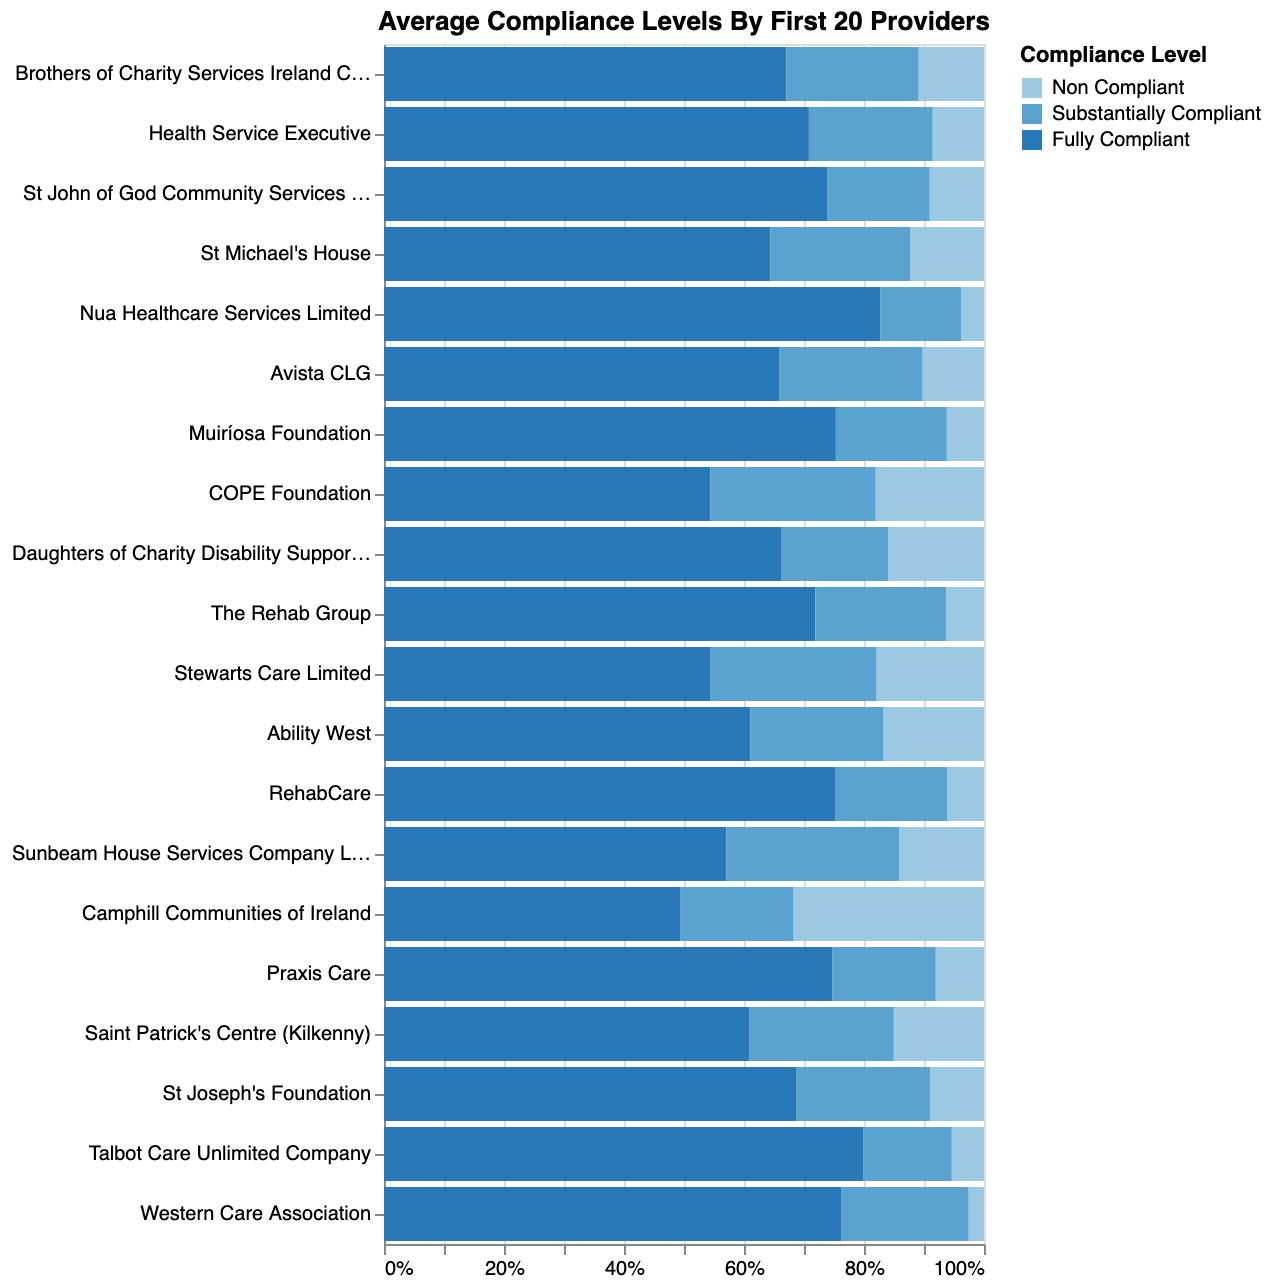
\includegraphics[width=.9\linewidth]{img/10_compliance_providers.png}
\end{center}

The Top 10 providers by \textbf{\% full compliance} were:

\begin{longtable}{p{10cm}|r|r}
\caption{Providers - \% Full Compliance}
\\[0pt]
Provider & Total Checked & \% Fully Compliant\\[0pt]
\hline
\endfirsthead
\multicolumn{3}{l}{Continued from previous page} \\[0pt]
\hline

Provider & Total Checked & \% Fully Compliant \\[0pt]

\hline
\endhead
\hline\multicolumn{3}{r}{Continued on next page} \\
\endfoot
\endlastfoot
\hline
The Multiple Sclerosis Society of Ireland & 13 & 100.0\\[0pt]
MyLife by Estrela Hall Limited & 87 & 95.8\\[0pt]
St. Paul's Child and Family Care Centre Designated Activity Company & 97 & 91.4\\[0pt]
Lorrequer House & 33 & 90.8\\[0pt]
Prosper Fingal Company Limited by Guarantee & 93 & 87.6\\[0pt]
Co Wexford Community Workshop (Enniscorthy) CLG & 76 & 84.6\\[0pt]
The Anne Sullivan Centre CLG & 36 & 81.1\\[0pt]
St Aidan's Day Care Centre Company Limited by Guarantee & 103 & 80.9\\[0pt]
Gheel Autism Services Company Limited by Guarantee & 112 & 79.0\\[0pt]
Terra Glen Residential Care Services Limited & 52 & 78.9\\[0pt]
 &  & \\[0pt]
\end{longtable}

The Top 10 providers by \textbf{\% full compliance where there were > 200 regulations checked} were:

\begin{longtable}{p{10cm}|r|r}
\caption{Providers - \% Full Compliance > 200 regulations checked}
\\[0pt]
Provider & Total Checked & \% Fully Compliant\\[0pt]
\hline
\endfirsthead
\multicolumn{3}{l}{Continued from previous page} \\[0pt]
\hline

Provider & Total Checked & \% Fully Compliant \\[0pt]

\hline
\endhead
\hline\multicolumn{3}{r}{Continued on next page} \\
\endfoot
\endlastfoot
\hline
GALRO Unlimited Company & 473 & 77.4\\[0pt]
Talbot Care Unlimited Company & 521 & 73.2\\[0pt]
RehabCare & 769 & 72.7\\[0pt]
Dundas Unlimited Company & 393 & 70.1\\[0pt]
Nua Healthcare Services Limited & 1814 & 70.1\\[0pt]
Western Care Association & 506 & 68.8\\[0pt]
Praxis Care & 634 & 66.1\\[0pt]
Daughters of Charity Disability Support Services CLG & 1222 & 63.9\\[0pt]
Muiríosa Foundation & 1515 & 63.0\\[0pt]
KARE, Promoting Inclusion for People with Intellectual Disabilities & 396 & 62.5\\[0pt]
 &  & \\[0pt]
\end{longtable}


As can be seen, \textbf{Nua Healthcare} stands out as a provider with both a high volume of inspections and a high level of compliance.
\section{Regulation 23: Governance and Management}
\label{sec:orgab3af12}

As Regulation 23: Governance and Management is both highly inspected and is approximately 20\% non compliant on average, it is worth looking more closely into it. From the HIQA documentation, the following elements contribute to this being marked as compliant/noncompliant:

Indicators of compliance include:

\begin{itemize}
\item the management structure is clearly defined and identifies the lines of authority and accountability, specifies roles and details responsibilities for all areas of service provision and includes arrangements for a person to manage the centre during absences of the person in charge, for example during annual leave or absence due to illness.
\item where there is more than one identified person participating in the management of the centre, the operational governance arrangement are clearly defined. Decisions are communicated, implemented and evaluated.
\item management systems are in place to ensure that the service provided is safe, appropriate to residents’ needs, consistent and effectively monitored
\item the person in charge demonstrates sufficient knowledge of the legislation and his/her statutory responsibilities and has complied with the regulations and or standards
\item there is an annual review of the quality and safety of care and support in the designated centre
\item a copy of the annual review is made available to residents
\item residents and their representatives are consulted with in the completion of the annual review of the quality and safety of care
\item the registered provider (or nominated person) visits the centre at least once every six months and produces a report on the safety and quality of care and support provided in the centre
\item arrangements are in place to ensure staff exercise their personal and professional responsibility for the quality and safety of the services that they are delivering
\item there are adequate resources to support residents achieving their individual personal plans
\item the facilities and services in the centre reflect the statement of purpose
\item practice is based on best practice and complies with legislative, regulatory and contractual requirements.
\end{itemize}

Indicators of non-compliance include:

\begin{itemize}
\item there are insufficient resources in the centre and the needs of residents are not met
\item there are sufficient resources but they are not appropriately managed to adequately meet residents’ needs
\item due to a lack of resources, the delivery of care and support is not in accordance with the statement of purpose
\item there is no defined management structure
\item governance and management systems are not known nor clearly defined
\item there are no clear lines of accountability for decision making and responsibility for the delivery of services to residents
\item staff are unaware of the relevant reporting mechanisms
\item there are no appropriate arrangements in place for periods when the person in charge is absence from the centre
\item the person in charge is absent from the centre but no suitable arrangements have been made for his or her absence
\item the person in charge is ineffective in his/her role and outcomes for residents are poor
\item the centre is managed by a suitably qualified person in charge; however, there are some gaps in his/her knowledge of their responsibilities under the regulations and this has resulted in some specific requirements not been met
\item the person in charge is inaccessible to residents and their families, and residents do not know who is in charge of the centre
\item an annual review of the quality and safety of care in the centre does not take place
\item an annual review of the quality and safety of care in the centre takes place but there is no evidence of learning from the review
\item a copy of the annual review is not made available to residents and or to the Chief Inspector
\item the registered provider (or nominated person) does not make an unannounced visit to the centre at least once every six months
\item the registered provider (or nominated person) does not produce a report on the safety and quality of care and support provided in the centre
\item effective arrangements are not in place to support, develop or manage all staff to exercise their responsibilities appropriately.
\end{itemize}
\subsection{By Year}
\label{sec:org222e6bc}
\begin{longtable}{rrrr}
\caption{Governance and Management by Year}
\\[0pt]
Year & Total & \% Not Compliant & \% Fully Compliant\\[0pt]
\hline
\endfirsthead
\multicolumn{4}{l}{Continued from previous page} \\[0pt]
\hline

Year & Total & \% Not Compliant & \% Fully Compliant \\[0pt]

\hline
\endhead
\hline\multicolumn{4}{r}{Continued on next page} \\
\endfoot
\endlastfoot
\hline
2023 & 562 & 21.35 & 48.93\\[0pt]
2022 & 686 & 19.10 & 49.71\\[0pt]
2021 & 1018 & 19.74 & 52.95\\[0pt]
2020 & 382 & 24.61 & 48.17\\[0pt]
\end{longtable}
\subsection{By Area}
\label{sec:org2eefaeb}
\begin{center}
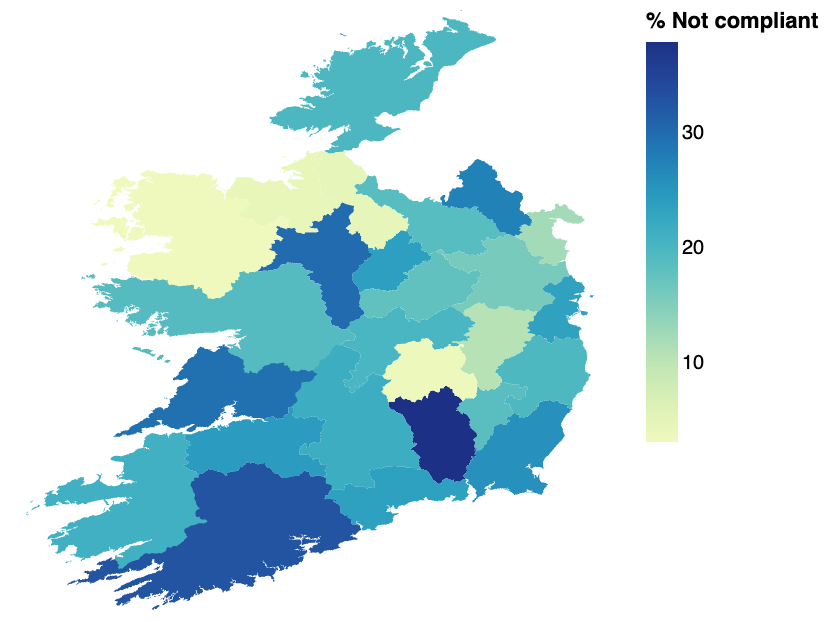
\includegraphics[width=.9\linewidth]{img/11_1_reg_23_percent_notitle.png}
\end{center}

\begin{longtable}{lrr}
\caption{Governance and Management \% Not Compliant (Dublin Grouped)}
\\[0pt]
Region & Total Checks for Governance & \% Non compliant\\[0pt]
\hline
\endfirsthead
\multicolumn{3}{l}{Continued from previous page} \\[0pt]
\hline

Region & Total Checks for Governance & \% Non compliant \\[0pt]

\hline
\endhead
\hline\multicolumn{3}{r}{Continued on next page} \\
\endfoot
\endlastfoot
\hline
Kilkenny & 132 & 37.88\\[0pt]
Cork & 207 & 32.85\\[0pt]
Roscommon & 40 & 30.00\\[0pt]
Clare & 75 & 29.33\\[0pt]
Monaghan & 40 & 27.50\\[0pt]
Wexford & 70 & 25.71\\[0pt]
Limerick & 140 & 24.29\\[0pt]
Longford & 21 & 23.81\\[0pt]
Waterford & 76 & 23.68\\[0pt]
Dublin & 524 & 23.00\\[0pt]
Tipperary & 88 & 21.59\\[0pt]
Kerry & 66 & 21.21\\[0pt]
Offaly & 45 & 20.00\\[0pt]
Donegal & 96 & 19.79\\[0pt]
Wicklow & 97 & 19.59\\[0pt]
Galway & 158 & 18.99\\[0pt]
Cavan & 16 & 18.75\\[0pt]
Carlow & 27 & 18.52\\[0pt]
Westmeath & 101 & 17.82\\[0pt]
Meath & 114 & 15.79\\[0pt]
Louth & 130 & 12.31\\[0pt]
Kildare & 150 & 10.67\\[0pt]
Leitrim & 21 & 4.76\\[0pt]
Sligo & 93 & 4.30\\[0pt]
Laois & 57 & 3.51\\[0pt]
Mayo & 64 & 3.13\\[0pt]
\end{longtable}


\begin{longtable}{lrr}
\caption{Governance and Management \% Not Compliant (Dublin Ungrouped)}
\\[0pt]
Region & Total Checks for Governance & \% Non compliant\\[0pt]
\hline
\endfirsthead
\multicolumn{3}{l}{Continued from previous page} \\[0pt]
\hline

Region & Total Checks for Governance & \% Non compliant \\[0pt]

\hline
\endhead
\hline\multicolumn{3}{r}{Continued on next page} \\
\endfoot
\endlastfoot
\hline
Dublin 17 & 3 & 66.67\\[0pt]
Dublin 4 & 2 & 50.00\\[0pt]
Dublin 10 & 2 & 50.00\\[0pt]
Dublin 15 & 61 & 42.62\\[0pt]
Dublin 8 & 5 & 40.00\\[0pt]
Kilkenny & 132 & 37.88\\[0pt]
Dublin 20 & 76 & 34.21\\[0pt]
Cork & 207 & 32.85\\[0pt]
Dublin 13 & 26 & 30.77\\[0pt]
Roscommon & 40 & 30.00\\[0pt]
Clare & 75 & 29.33\\[0pt]
Monaghan & 40 & 27.50\\[0pt]
Wexford & 70 & 25.71\\[0pt]
Dublin 7 & 40 & 25.00\\[0pt]
Dublin 3 & 8 & 25.00\\[0pt]
Limerick & 140 & 24.29\\[0pt]
Longford & 21 & 23.81\\[0pt]
Waterford & 76 & 23.68\\[0pt]
Dublin 5 & 34 & 23.53\\[0pt]
Dublin 18 & 9 & 22.22\\[0pt]
Tipperary & 88 & 21.59\\[0pt]
Kerry & 66 & 21.21\\[0pt]
Dublin 6w & 25 & 20.00\\[0pt]
Offaly & 45 & 20.00\\[0pt]
Dublin 14 & 20 & 20.00\\[0pt]
Donegal & 96 & 19.79\\[0pt]
Wicklow & 97 & 19.59\\[0pt]
Galway & 158 & 18.99\\[0pt]
Cavan & 16 & 18.75\\[0pt]
Carlow & 27 & 18.52\\[0pt]
Westmeath & 101 & 17.82\\[0pt]
Meath & 114 & 15.79\\[0pt]
Louth & 130 & 12.31\\[0pt]
Dublin 22 & 9 & 11.11\\[0pt]
Kildare & 150 & 10.67\\[0pt]
Co. Dublin & 105 & 9.52\\[0pt]
Dublin 16 & 14 & 7.14\\[0pt]
Dublin 24 & 14 & 7.14\\[0pt]
Dublin 9 & 49 & 6.12\\[0pt]
Leitrim & 21 & 4.76\\[0pt]
Sligo & 93 & 4.30\\[0pt]
Laois & 57 & 3.51\\[0pt]
Mayo & 64 & 3.13\\[0pt]
Dublin 11 & 10 & 0.00\\[0pt]
Dublin 12 & 11 & 0.00\\[0pt]
Dublin 6 & 1 & 0.00\\[0pt]
\end{longtable}


\begin{longtable}{lrrr}
\caption{Governance and Management - 2023 Only}
\\[0pt]
Region & Total Checks for Governance & \% Non compliant & \% Fully compliant\\[0pt]
\hline
\endfirsthead
\multicolumn{4}{l}{Continued from previous page} \\[0pt]
\hline

Region & Total Checks for Governance & \% Non compliant & \% Fully compliant \\[0pt]

\hline
\endhead
\hline\multicolumn{4}{r}{Continued on next page} \\
\endfoot
\endlastfoot
\hline
Galway & 41 & 51.22 & 34.15\\[0pt]
Cork & 54 & 46.30 & 9.26\\[0pt]
Roscommon & 8 & 37.50 & 25.00\\[0pt]
Kilkenny & 26 & 34.62 & 34.62\\[0pt]
Clare & 18 & 33.33 & 55.56\\[0pt]
Limerick & 35 & 22.86 & 45.71\\[0pt]
Waterford & 23 & 21.74 & 52.17\\[0pt]
Leitrim & 6 & 16.67 & 33.33\\[0pt]
Meath & 26 & 15.38 & 65.38\\[0pt]
Westmeath & 26 & 15.38 & 65.38\\[0pt]
Wicklow & 20 & 15.00 & 35.00\\[0pt]
Monaghan & 7 & 14.29 & 42.86\\[0pt]
Longford & 7 & 14.29 & 57.14\\[0pt]
Kildare & 22 & 13.64 & 63.64\\[0pt]
Donegal & 22 & 13.64 & 27.27\\[0pt]
Offaly & 8 & 12.50 & 62.50\\[0pt]
Tipperary & 16 & 12.50 & 75.00\\[0pt]
Louth & 33 & 12.12 & 66.67\\[0pt]
Laois & 10 & 10.00 & 40.00\\[0pt]
Mayo & 10 & 10.00 & 60.00\\[0pt]
Wexford & 11 & 9.09 & 81.82\\[0pt]
Dublin & 92 & 8.00 & 50.00\\[0pt]
Sligo & 20 & 5.00 & 60.00\\[0pt]
Cavan & 2 & 0.00 & 50.00\\[0pt]
Carlow & 5 & 0.00 & 80.00\\[0pt]
Kerry & 14 & 0.00 & 71.43\\[0pt]
\end{longtable}
\subsection{By Provider}
\label{sec:orgbba8fec}

\subsubsection{Highest \% Fully Compliant}
\label{sec:org1956a71}
\begin{center}
\begin{tabular}{lrr}
Provider & Total & \% Fully compliant\\[0pt]
\hline
Dara Residential Services & 9 & 100.0\\[0pt]
Co Wexford Community Workshop (Enniscorthy) CLG & 6 & 100.0\\[0pt]
MyLife by Estrela Hall Limited & 6 & 100.0\\[0pt]
Redwood Neurobehavioural Services Unlimited Company & 4 & 100.0\\[0pt]
Lorrequer House & 2 & 100.0\\[0pt]
The Anne Sullivan Centre CLG & 2 & 100.0\\[0pt]
St. Aidan's Day Care Centre Company Limited by Guarantee & 1 & 100.0\\[0pt]
Positive Futures: Achieving Dreams. Transforming Lives. CLG & 1 & 100.0\\[0pt]
IRL-IASD CLG & 1 & 100.0\\[0pt]
The Multiple Sclerosis Society of Ireland & 1 & 100.0\\[0pt]
\end{tabular}
\end{center}
\subsubsection{Highest \% Fully Compliant with > 50 Inspections}
\label{sec:orgffc61ab}

\begin{center}
\begin{tabular}{lrrr}
Provider & Total & \% Not compliant & \% Fully compliant\\[0pt]
\hline
Nua Healthcare Services Limited & 128 & 4.7 & 77.3\\[0pt]
St John of God Community Services CLG & 188 & 11.2 & 68.1\\[0pt]
Muiríosa Foundation & 95 & 8.4 & 66.3\\[0pt]
RehabCare & 51 & 15.7 & 58.8\\[0pt]
The Rehab Group & 63 & 12.7 & 57.1\\[0pt]
St Michael's House & 155 & 18.7 & 56.8\\[0pt]
Avista CLG & 102 & 18.6 & 48.0\\[0pt]
Stewarts Care Limited & 68 & 33.8 & 45.6\\[0pt]
Health Service Executive & 303 & 17.5 & 44.9\\[0pt]
Brothers of Charity Services Ireland CLG & 346 & 26.0 & 40.5\\[0pt]
\end{tabular}
\end{center}
\subsubsection{Highest \% Not Compliant}
\label{sec:org9f3b61c}

\begin{center}
\begin{tabular}{lrr}
Provider & Total & \% Not compliant\\[0pt]
\hline
Redwood Neurobehavioral Services Unlimited Company & 1 & 100.0\\[0pt]
Asperger Syndrome Association of Ireland CLG & 1 & 100.0\\[0pt]
Ard Aoibhinn Community Initiatives CLG & 3 & 66.7\\[0pt]
Stepping Stones Residential Care Limited & 7 & 57.1\\[0pt]
Camphill Communities of Ireland & 55 & 52.7\\[0pt]
Saint Patrick's Centre (Kilkenny) & 10 & 50.0\\[0pt]
Bradbury House Ireland Limited & 2 & 50.0\\[0pt]
Peacehaven Trust CLG & 2 & 50.0\\[0pt]
St Catherine's Association CLG & 2 & 50.0\\[0pt]
MooreHaven Centre (Tipperary) Designated Activity Company & 2 & 50.0\\[0pt]
\end{tabular}
\end{center}
\subsubsection{Highest \% Not Compliant with > 50 Inspections}
\label{sec:org5115a17}

\begin{center}
\begin{tabular}{lrr}
Provider & Total & \% Not compliant\\[0pt]
\hline
Camphill Communities of Ireland & 55 & 52.7\\[0pt]
COPE Foundation & 83 & 48.2\\[0pt]
Ability West & 69 & 40.6\\[0pt]
Daughters of Charity Disability Support Services CLG & 88 & 35.2\\[0pt]
Stewarts Care Limited & 68 & 33.8\\[0pt]
Sunbeam House Services Company Limited by Guarantee & 56 & 26.8\\[0pt]
Brothers of Charity Services Ireland CLG & 346 & 26.0\\[0pt]
St Michael's House & 155 & 18.7\\[0pt]
Avista CLG & 102 & 18.6\\[0pt]
Health Service Executive & 303 & 17.5\\[0pt]
\end{tabular}
\end{center}
\section{Sentiment (Experimental)}
\label{sec:org7e318e0}

Aggregate 'sentiment' levels were obtained by passing the text contained under the section \textbf{\textbf{What residents told us and what inspectors observed}} to \texttt{GPT-3.5} for evaluation.

The following prompt was provided:

\begin{quote}
Summarize the following text into 5 keywords reflecting the sentiment of the residents. Do not include the word 'residents' as a keyword.

Also provide 3 key phrases reflecting the sentiment of the residents

Also assign an overall rating of 'positive', 'negative' or 'neutral' based on these sentiments.

Finally, summarise the text in two sentences.
\end{quote}

In other words, the following was asked for:

\begin{itemize}
\item \textbf{\textbf{rating}} (positive/negative/neutral)
\item \textbf{\textbf{keywords}} (5)
\item \textbf{\textbf{key phrases}} (3)
\item \textbf{\textbf{summary}} (2 sentences)
\end{itemize}

There are a couple of major caveats here:

\begin{enumerate}
\item I used the least powerful version of GPT. The cost was around \$6.69 for 3,733 requests (this included some trail and error requests at the outset). The next most powerful api (\texttt{GPT-4}) would have cost around 30x this.
\item This was more of a 'proof of concept' exercise, more work would need to be done on the specfics of the GPT model, especially questions around how best to formulate the prompt. This exercise was primarily exploratory in nature, therefore a limited amount of time was spent engineering the prompt.
\end{enumerate}

The total word count across all the observation sections of the reports was approximately \textbf{2,550,376} words. The average word count for the observation sections of the reports was \textbf{802.26} words.
\subsection{Rating}
\label{sec:org4eddb74}

\textbf{86\%} of the inspections received a ``positive'' rating by the GPT model, based on the text containing observations of the inspections and what the residents said about the centre.

Across inspections in 2021, 2022, and 2023 (the years with most inspections), the percentage of ``negatively'' rated centres was around \textbf{10-11\%}.

\begin{center}
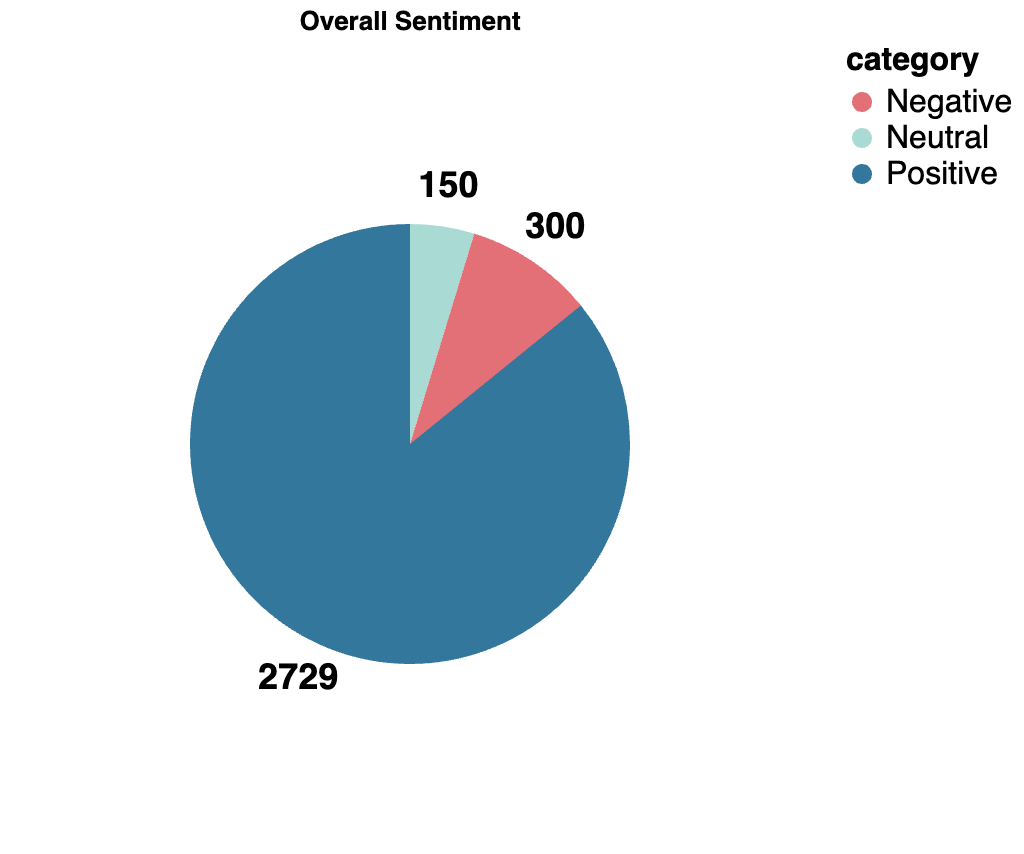
\includegraphics[width=.9\linewidth]{img/14_rating_pie.png}
\end{center}

\begin{center}
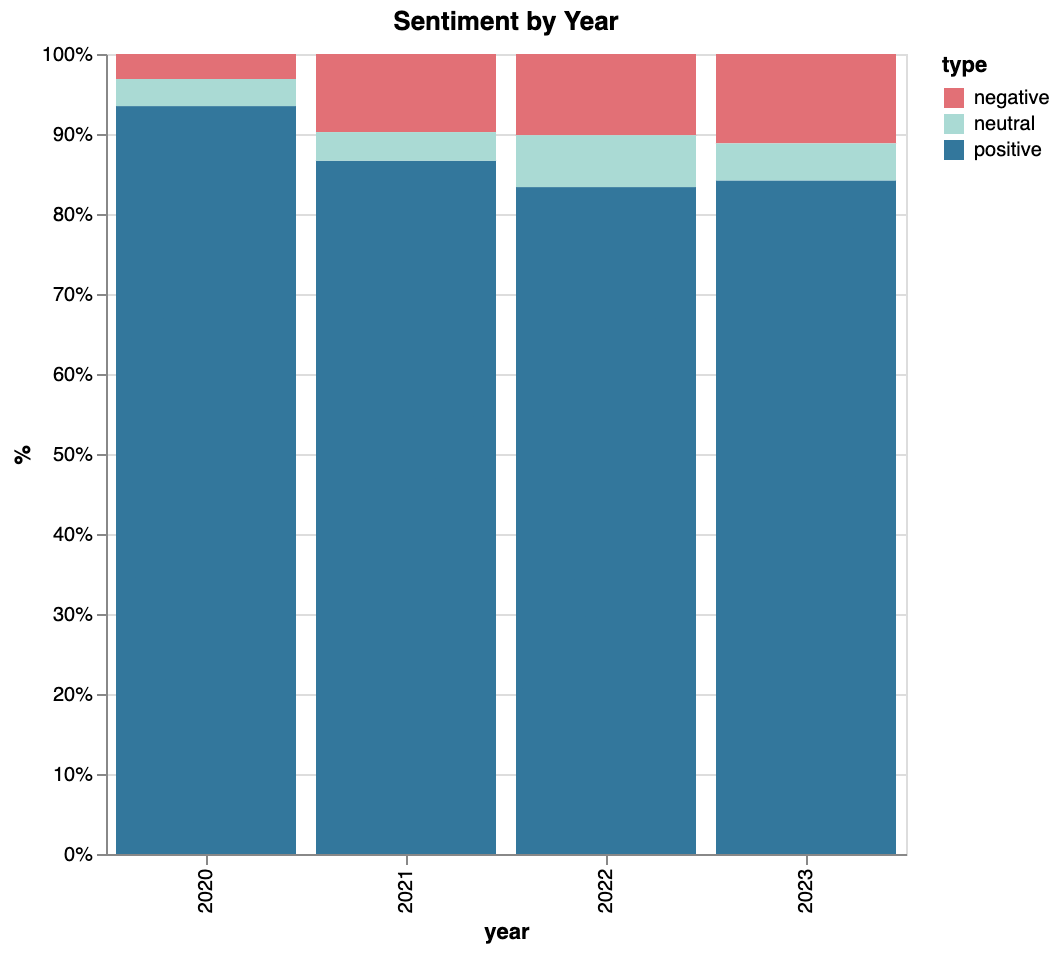
\includegraphics[width=12cm]{img/15_rating_year.png}
\end{center}

\begin{center}
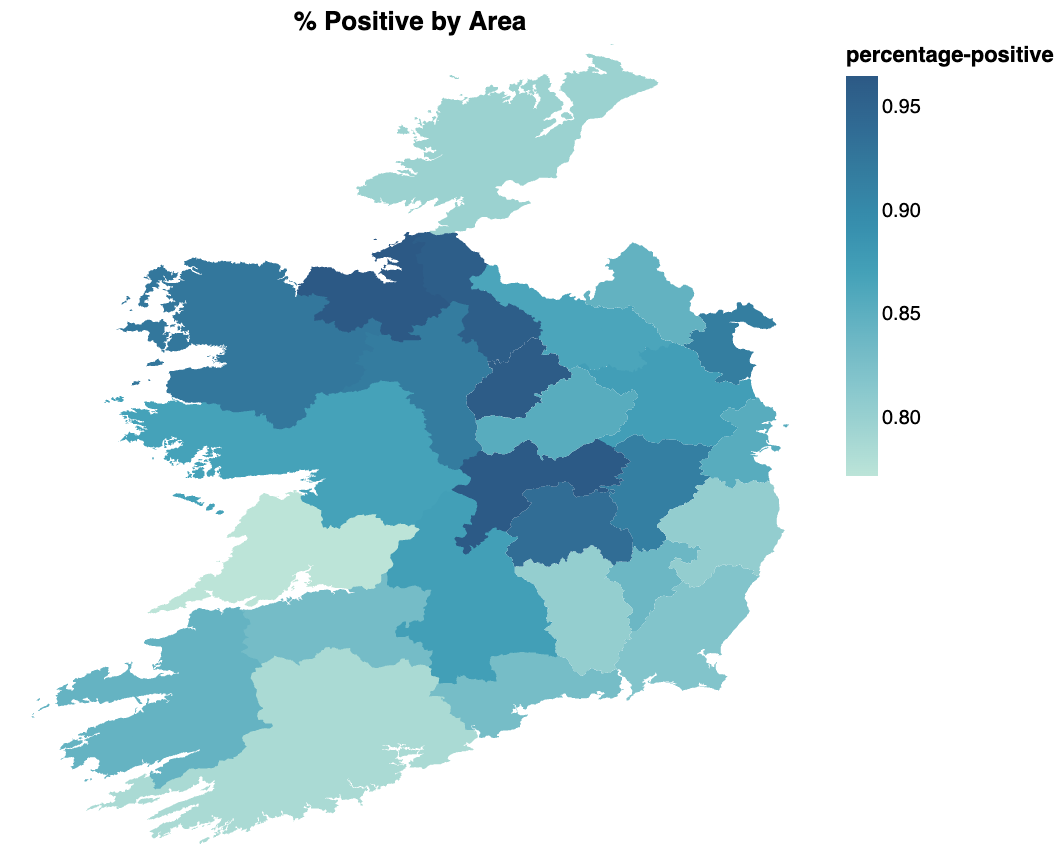
\includegraphics[width=.9\linewidth]{img/16_rating_area.png}
\end{center}

These ratings also align with average levels of compliance. Centres with a ``positive'' rating were on average \textbf{73\%} fully compliant and \textbf{7\%} not compliant. Centres with a ``negative'' rating were on average \textbf{34\%} fully compliant and \textbf{43\%} not compliant. Therefore, accepting the limitations of this approach, you could conclude from these AI ratings that higher levels of compliance with the HIQA regulations leads to better user experience.

There is also a very tentative alignment between ``positive'' ratings and ``number of residents present''. As can be seen below, ``positive'' sentiment trends slightly downward in the case of more residents.

\begin{center}
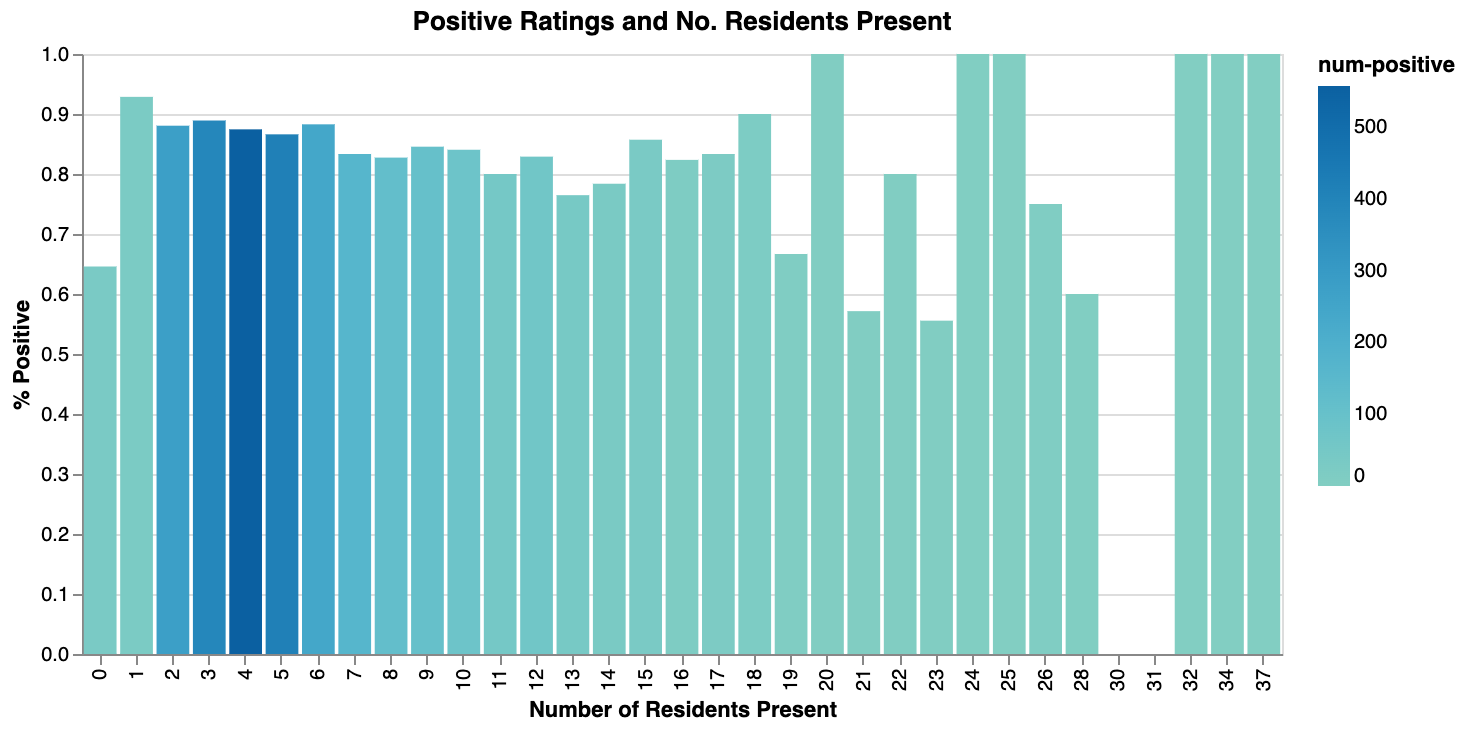
\includegraphics[width=.9\linewidth]{img/17_rating_residents_pos.png}
\end{center}

\begin{center}
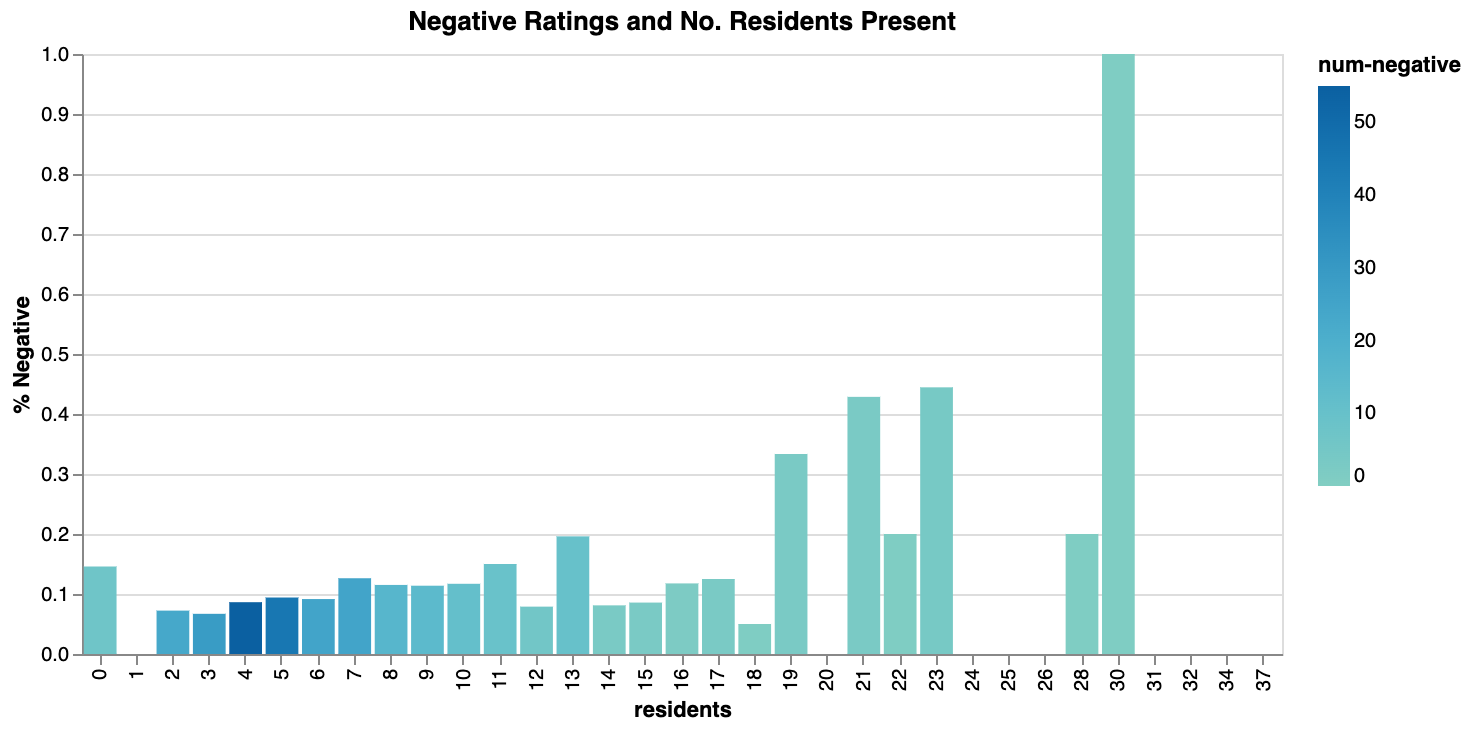
\includegraphics[width=.9\linewidth]{img/18_rating_res_neg.png}
\end{center}
\subsection{Keywords and Key Phrases}
\label{sec:org31a9aee}

The top 5 most frequent keywords for centres with a ``positive'' rating were \textbf{support}, \textbf{happy}, \textbf{comfortable}, \textbf{activities}, and \textbf{staff}. The top 5 keywords for centres with a ``negative'' rating were \textbf{infection prevention and control}, \textbf{compliance}, \textbf{improvements}, \textbf{staff}, and \textbf{support}. As can be seen, the word ``staff'' features prominently in both ``negative'' and ``positively'' rated centres, suggesting that staff are a key feature in shaping sentiment.

The top 10 most frequent key phrases that appeared were:

\begin{enumerate}
\item Good quality of life
\item Improvements were required
\item Residents were happy
\item Residents were supported
\item Residents appeared comfortable
\item Liked living in the centre
\item Residents felt safe
\item Unannounced Inspection
\item Warm interactions between residents and staff
\item Clean and tidy
\end{enumerate}
\subsubsection{Word Clouds}
\label{sec:orgd3473dc}

Below is a word cloud for the keywords associated with \textbf{positively} rated centres:

\begin{center}
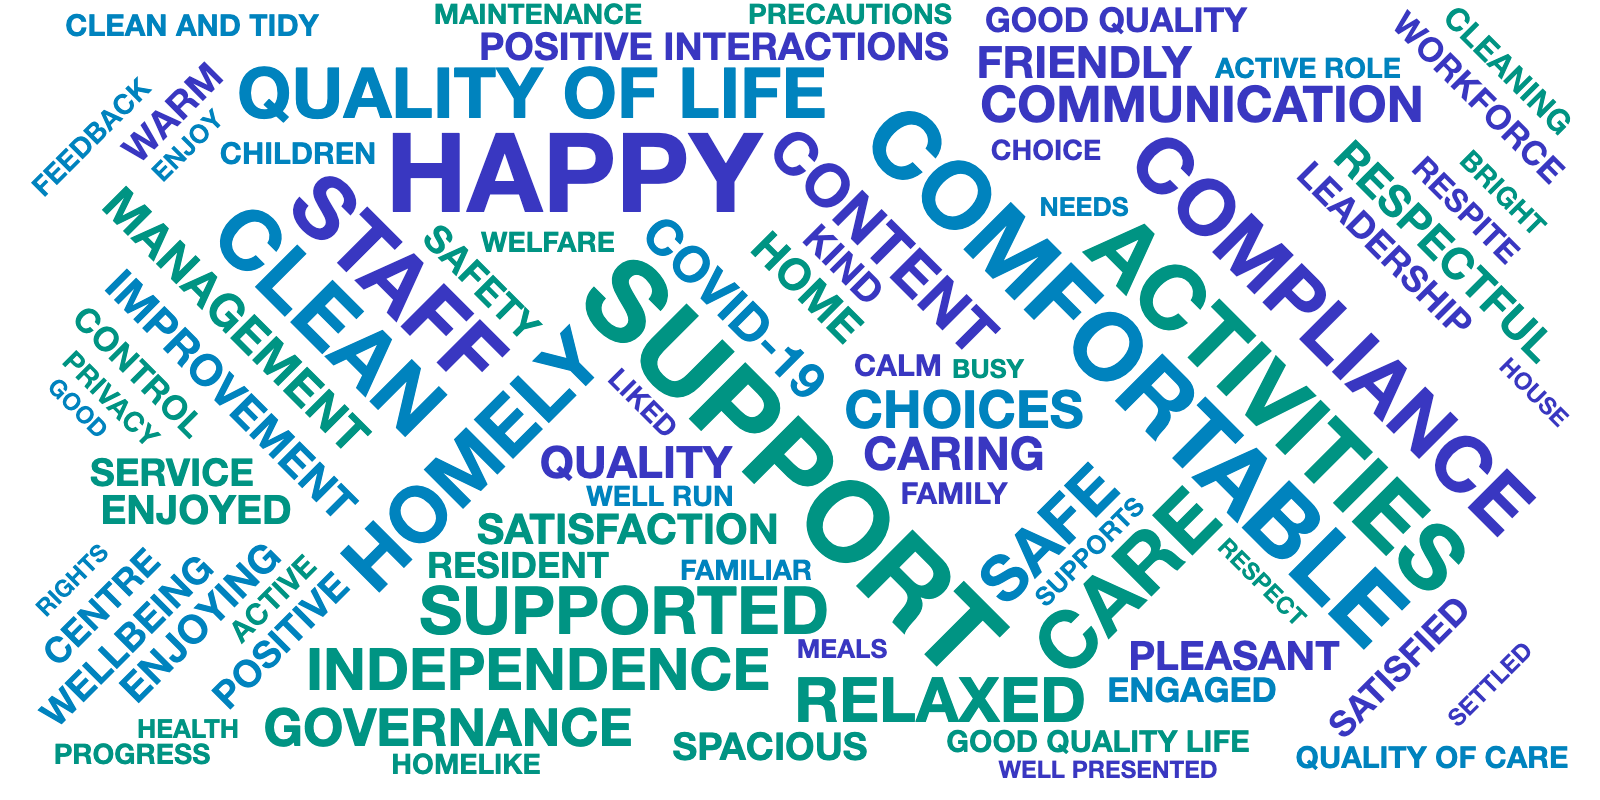
\includegraphics[width=.9\linewidth]{img/19_word_cloud_pos.png}
\end{center}

A word cloud for the keywords associated with \textbf{negatively} rated centres:

\begin{center}
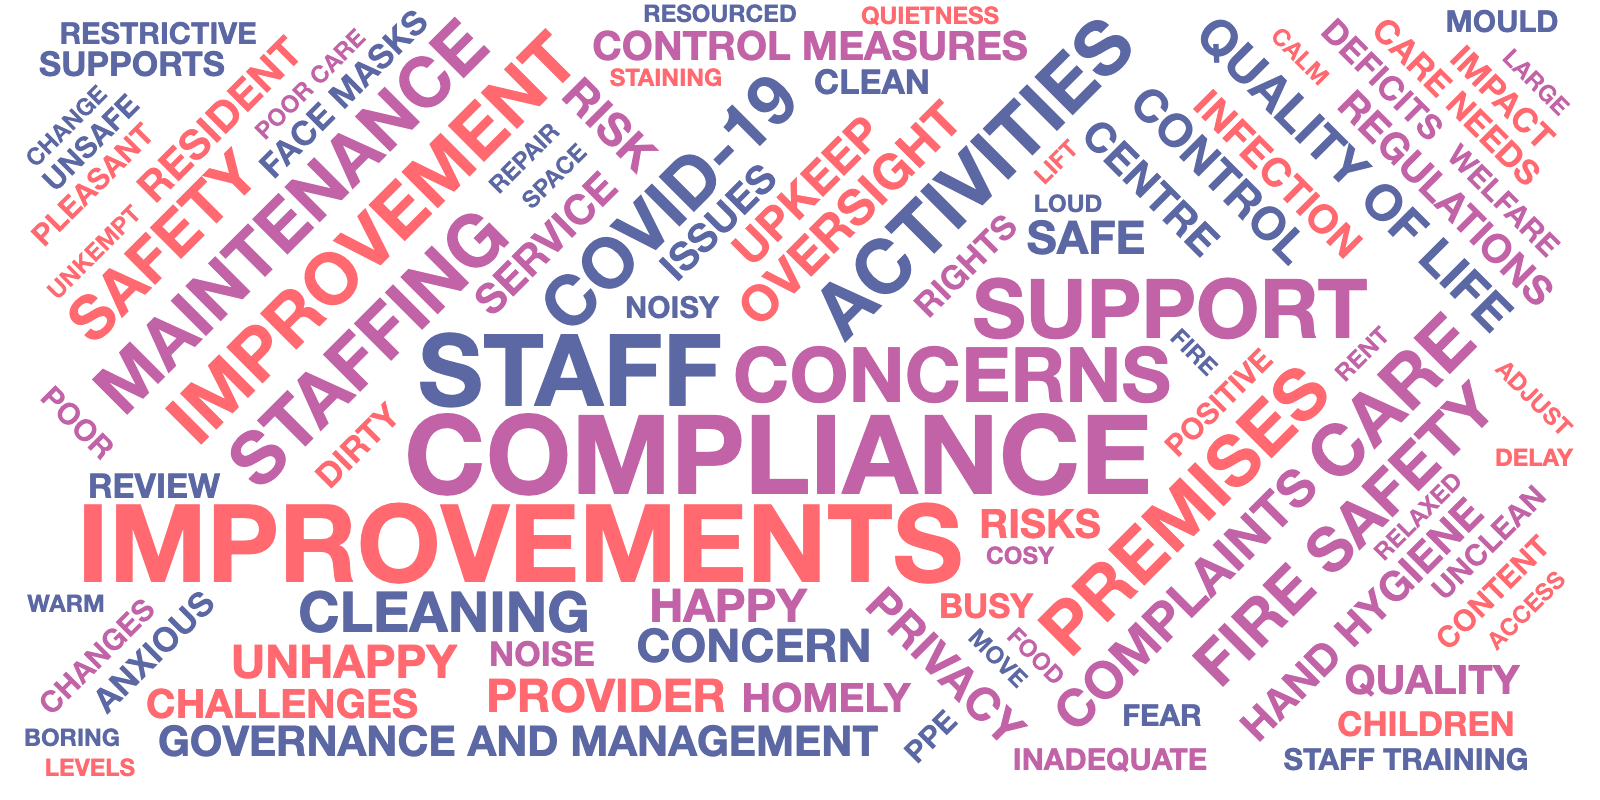
\includegraphics[width=.9\linewidth]{img/20_word_cloud_neg.png}
\end{center}
\subsection{Summaries}
\label{sec:orgd99ca34}

Below are some \textbf{randomized} examples of GPT ``summaries'', along with a link to the reports and some additional details for context.
\subsubsection{A report from 2023}
\label{sec:orgc3fe639}

\textbf{Summary} :: The residents of this care center are very happy and speak highly of the supportive staff. The center provides a comfortable and warm living environment, and the staff actively work to maximize residents' social care and independence.

\href{https://www.hiqa.ie/system/files?file=inspectionreports/3702-mountain-view-residential-respite-services-16-january-2023.pdf}{Full Report Link}

\begin{longtable}{p{11cm}|p{5cm}}
Heading & Information\\[0pt]
\hline
\endfirsthead
\multicolumn{2}{l}{Continued from previous page} \\[0pt]
\hline

Heading & Information \\[0pt]

\hline
\endhead
\hline\multicolumn{2}{r}{Continued on next page} \\
\endfoot
\endlastfoot
\hline
Centre id & 3702\\[0pt]
Date & 2023-01-16\\[0pt]
Name of provider & Western Care Association\\[0pt]
Address of centre & Mayo\\[0pt]
Number of residents present & 8\\[0pt]
Type of inspection & Announced\\[0pt]
Percent noncompliant & 0.000\\[0pt]
Rating & positive\\[0pt]
Regulation 08: Protection (Quality and safety) & Compliant\\[0pt]
Regulation 10: Communication (Quality and safety) & Compliant\\[0pt]
Regulation 15: Staffing (Capacity and capability) & Compliant\\[0pt]
Regulation 05: Individualised assessment and personal plan (Quality and safety) & Compliant\\[0pt]
Regulation 31: Notification of incidents (Capacity and capability) & Compliant\\[0pt]
Regulation 03: Statement of purpose (Capacity and capability) & Compliant\\[0pt]
Regulation 06: Healthcare (Quality and safety) & Compliant\\[0pt]
Regulation 20: Information for residents (Quality and safety) & Compliant\\[0pt]
Regulation 28: Fire precautions (Quality and safety) & Compliant\\[0pt]
Regulation 09: Residents' rights (Quality and safety) & Compliant\\[0pt]
Regulation 07: Positive behaviour support (Quality and safety) & Compliant\\[0pt]
Regulation 26: Risk management procedures (Quality and safety) & Compliant\\[0pt]
Regulation 16: Training and staff development (Capacity and capability) & Compliant\\[0pt]
Regulation 23: Governance and management (Capacity and capability) & Compliant\\[0pt]
Regulation 17: Premises (Quality and safety) & Compliant\\[0pt]
Regulation 11: Visits (Quality and safety) & Compliant\\[0pt]
Regulation 14: Person in charge (Capacity and capability) & Compliant\\[0pt]
\end{longtable}
\subsubsection{A report for a Congregated Setting}
\label{sec:org969bf0b}

\textbf{Summary} :: The residents were supportive and enjoyed various activities during the inspection, such as having nail varnish applied and receiving a hand massage. They also expressed their desire to move out of the designated center and have their own apartment.

\href{https://www.hiqa.ie/system/files?file=inspectionreports/4745-lios-mor-16-september-2020.pdf}{Full Report Link}

\begin{longtable}{p{11cm}|p{5cm}}
Heading & Information\\[0pt]
\hline
\endfirsthead
\multicolumn{2}{l}{Continued from previous page} \\[0pt]
\hline

Heading & Information \\[0pt]

\hline
\endhead
\hline\multicolumn{2}{r}{Continued on next page} \\
\endfoot
\endlastfoot
\hline
Centre id & 4745\\[0pt]
Date & 2020-09-16\\[0pt]
Name of provider & Brothers of Charity Services Ireland CLG\\[0pt]
Address of centre & Limerick\\[0pt]
Number of residents present & 10\\[0pt]
Type of inspection & Short Notice Announced\\[0pt]
Percent noncompliant & 5.263\\[0pt]
Rating & positive\\[0pt]
Regulation 08: Protection (Quality and safety) & Substantially compliant\\[0pt]
Regulation 27: Protections against infection (Quality and safety) & Substantially compliant\\[0pt]
Regulation 10: Communication (Quality and safety) & Compliant\\[0pt]
Regulation 15: Staffing (Capacity and capability) & Compliant\\[0pt]
Regulation 34: Complaints procedure (Capacity and capability) & Compliant\\[0pt]
Regulation 05: Individualised assessment and personal plan (Quality and safety) & Compliant\\[0pt]
Regulation 31: Notification of incidents (Capacity and capability) & Not compliant\\[0pt]
Regulation 03: Statement of purpose (Capacity and capability) & Compliant\\[0pt]
Regulation 06: Healthcare (Quality and safety) & Compliant\\[0pt]
Regulation 20: Information for residents (Quality and safety) & Compliant\\[0pt]
Regulation 28: Fire precautions (Quality and safety) & Substantially compliant\\[0pt]
Regulation 09: Residents' rights (Quality and safety) & Compliant\\[0pt]
Regulation 07: Positive behaviour support (Quality and safety) & Compliant\\[0pt]
Regulation 26: Risk management procedures (Quality and safety) & Substantially compliant\\[0pt]
Regulation 16: Training and staff development (Capacity and capability) & Compliant\\[0pt]
Regulation 23: Governance and management (Capacity and capability) & Compliant\\[0pt]
Regulation 13: General welfare and development (Quality and safety) & Compliant\\[0pt]
Regulation 11: Visits (Quality and safety) & Compliant\\[0pt]
Regulation 14: Person in charge (Capacity and capability) & Compliant\\[0pt]
\end{longtable}
\subsubsection{A report for an inspection with a 'negative' GPT rating}
\label{sec:orgd6693fb}

\textbf{Summary} :: The residents have positive and active lifestyles. However, the inspection found issues with falls hazards, risk management, and staffing arrangements.

\href{https://www.hiqa.ie/system/files?file=inspectionreports/1495-ocean-wave-services-04-july-2023.pdf}{Full Report Link}


\begin{longtable}{p{11cm}|p{5cm}}
Heading & Information\\[0pt]
\hline
\endfirsthead
\multicolumn{2}{l}{Continued from previous page} \\[0pt]
\hline

Heading & Information \\[0pt]

\hline
\endhead
\hline\multicolumn{2}{r}{Continued on next page} \\
\endfoot
\endlastfoot
\hline
Centre id & 1495\\[0pt]
Date & 2023-07-04\\[0pt]
Name of provider & Ability West\\[0pt]
Address of centre & Galway\\[0pt]
Number of residents present & 4\\[0pt]
Type of inspection & Unannounced\\[0pt]
Percent noncompliant & 60.00\\[0pt]
Rating & negative\\[0pt]
Regulation 15: Staffing (Capacity and capability) & Not compliant\\[0pt]
Regulation 14: Person in charge (Capacity and capability) & Compliant\\[0pt]
Regulation 05: Individualised assessment and personal plan (Quality and safety) & Compliant\\[0pt]
Regulation 23: Governance and management (Capacity and capability) & Not compliant\\[0pt]
Regulation 26: Risk management procedures (Quality and safety) & Not compliant\\[0pt]
\end{longtable}
\subsubsection{A report for a centre with > 50\% non compliance}
\label{sec:org3f8c663}

\textbf{Summary} :: The residents expressed a mixed sentiment about the center, with some enjoying their time there and others lamenting the restrictions due to COVID-19. Inspectors found shortcomings in infection prevention measures, including incorrect use of face masks and expired alcohol gel bottles. The overall rating is negative, as improvements are needed in various areas.

\href{https://www.hiqa.ie/system/files?file=inspectionreports/2036-ard-na-mara-15-february-2022.pdf}{Full Report Link}


\begin{longtable}{p{11cm}|p{5cm}}
Heading & Information\\[0pt]
\hline
\endfirsthead
\multicolumn{2}{l}{Continued from previous page} \\[0pt]
\hline

Heading & Information \\[0pt]

\hline
\endhead
\hline\multicolumn{2}{r}{Continued on next page} \\
\endfoot
\endlastfoot
\hline
Centre id & 2036\\[0pt]
Date & 2022-02-15\\[0pt]
Name of provider & Enable Ireland Disability Services Limited\\[0pt]
Address of centre & Cork\\[0pt]
Number of residents present & 5\\[0pt]
Type of inspection & Unannounced\\[0pt]
Percent noncompliant & 100.0\\[0pt]
Rating & negative\\[0pt]
Regulation 27: Protections against infection (Quality and safety) & Not compliant\\[0pt]
\end{longtable}
\subsubsection{A report for a centre with 'staffing' keyword and 'negative' rating}
\label{sec:org01855bb}

\textbf{Summary} :: Residents were generally happy living in the centre and felt safe, but there were areas that required improvement. These included premises, restrictive practices, staffing, and management arrangements.

\href{https://www.hiqa.ie/system/files?file=inspectionreports/7820-tonyglassion-group-home-28-january-2021.pdf}{Full Report Link}


\begin{longtable}{p{11cm}|p{5cm}}
Heading & Information\\[0pt]
\hline
\endfirsthead
\multicolumn{2}{l}{Continued from previous page} \\[0pt]
\hline

Heading & Information \\[0pt]

\hline
\endhead
\hline\multicolumn{2}{r}{Continued on next page} \\
\endfoot
\endlastfoot
\hline
Centre id & 7820\\[0pt]
Date & 2021-01-28\\[0pt]
Name of provider & Health Service Executive\\[0pt]
Address of centre & Monaghan\\[0pt]
Number of residents present & 5\\[0pt]
Type of inspection & Short Notice Announced\\[0pt]
Percent noncompliant & 41.67\\[0pt]
Rating & negative\\[0pt]
Regulation 08: Protection (Quality and safety) & Compliant\\[0pt]
Regulation 27: Protections against infection (Quality and safety) & Compliant\\[0pt]
Regulation 15: Staffing (Capacity and capability) & Not compliant\\[0pt]
Regulation 34: Complaints procedure (Capacity and capability) & Compliant\\[0pt]
Regulation 31: Notification of incidents (Capacity and capability) & Compliant\\[0pt]
Regulation 28: Fire precautions (Quality and safety) & Substantially compliant\\[0pt]
Regulation 09: Residents' rights (Quality and safety) & Not compliant\\[0pt]
Regulation 07: Positive behaviour support (Quality and safety) & Not compliant\\[0pt]
Regulation 16: Training and staff development (Capacity and capability) & Compliant\\[0pt]
Regulation 23: Governance and management (Capacity and capability) & Not compliant\\[0pt]
Regulation 17: Premises (Quality and safety) & Not compliant\\[0pt]
Regulation 14: Person in charge (Capacity and capability) & Compliant\\[0pt]
\end{longtable}
\subsubsection{A report for a centre with 'staffing' keyword and 'positive' rating}
\label{sec:orgcba7ac9}

\textbf{Summary} :: Residents living in the Orchid Lane designated centre are generally happy with their living environment and the support they receive. They enjoy the amenities and services close by, have varied care needs, and receive appropriate supports. Some residents have unresolved concerns, but overall, the quality and safety of the service has improved, with enhancements to fire safety systems being made. Staffing deficits pose a risk to the service, but residents feel that their needs are being met.

\href{https://www.hiqa.ie/system/files?file=inspectionreports/5052-orchid-lane-04-april-2023.pdf}{Full Report Link}

\begin{longtable}{p{11cm}|p{5cm}}
Heading & Information\\[0pt]
\hline
\endfirsthead
\multicolumn{2}{l}{Continued from previous page} \\[0pt]
\hline

Heading & Information \\[0pt]

\hline
\endhead
\hline\multicolumn{2}{r}{Continued on next page} \\
\endfoot
\endlastfoot
\hline
Centre id & 5052\\[0pt]
Date & 2023-04-04\\[0pt]
Name of provider & Sunbeam House Services Company Limited by Guarantee\\[0pt]
Address of centre & Wicklow\\[0pt]
Number of residents present & 4\\[0pt]
Type of inspection & Unannounced\\[0pt]
Percent noncompliant & 9.091\\[0pt]
Rating & positive\\[0pt]
Regulation 08: Protection (Quality and safety) & Compliant\\[0pt]
Regulation 27: Protections against infection (Quality and safety) & Substantially compliant\\[0pt]
Regulation 15: Staffing (Capacity and capability) & Not compliant\\[0pt]
Regulation 05: Individualised assessment and personal plan (Quality and safety) & Substantially compliant\\[0pt]
Regulation 03: Statement of purpose (Capacity and capability) & Compliant\\[0pt]
Regulation 24: Admissions and contract for the provision of services (Capacity and capability) & Substantially compliant\\[0pt]
Regulation 28: Fire precautions (Quality and safety) & Substantially compliant\\[0pt]
Regulation 07: Positive behaviour support (Quality and safety) & Substantially compliant\\[0pt]
Regulation 16: Training and staff development (Capacity and capability) & Compliant\\[0pt]
Regulation 23: Governance and management (Capacity and capability) & Compliant\\[0pt]
Regulation 14: Person in charge (Capacity and capability) & Compliant\\[0pt]
\end{longtable}

\clearpage
\appendix
\section{Appendix - Dataset Info}
\label{sec:org5818e7c}

The main dataset created from the parsing of the reports can be found at in \href{https://github.com/loopdreams/inspection-reports-hiqa/blob/main/resources/datasets/created/pdf\_data\_full.csv}{csv form on github}.

Below is a list of the column headings:

\begin{center}
\begin{tabularx}{\textwidth}{XXXXXX}
\hline
Column Name & :n-missing & :min & :mean & :mode & :max\\[0pt]
\hline
\hline
:centre-id & 0 & 1388 & 4495 &  & 8475\\[0pt]
\hline
:centre-ID-OSV & 0 &  &  & OSV-0005490 & \\[0pt]
\hline
:year & 0 & 2020 & 2022 &  & 2023\\[0pt]
\hline
:date-of-inspection & 0 &  &  & 05 October 2021 & \\[0pt]
\hline
:report-id & 0 &  &  & 7925-20230814 & \\[0pt]
\hline
:name-of-designated-centre & 0 &  &  & The Willows & \\[0pt]
\hline
:address-of-centre & 0 &  &  & Cork & \\[0pt]
\hline
:name-of-provider & 0 &  &  & Brothers of Charity Services Ireland CLG & \\[0pt]
\hline
:type-of-inspection & 0 &  &  & Unannounced & \\[0pt]
\hline
:number-of-residents-present & 41 & 0.000 & 5.960 &  & 37.00\\[0pt]
\hline
:date & 0 & 2020-06-03 & 2022-02-27 &  & 2023-10-18\\[0pt]
\hline
:report-URL & 19 &  &  &  & \\[0pt]
\hline
:fieldwork-ID & 0 &  &  & MON-0029506 & \\[0pt]
\hline
\end{tabularx}
\end{center}


There are also 33 columns relating to the regulations and one column containing the long text from the 'observations' section.

The columns \texttt{:report-id} and \texttt{:date} were manually added. \texttt{:report-id} was created as a unique identifier and combines the centre id followed by a hyphen ``-'' and the date of inspection in ``yyyyddmm'' format. In some cases inspections took place across two dates. In these cases the latter date was chosen for the \texttt{:date} and \texttt{:report-id} columns.
\end{document}
